%% This is an example first chapter.  You should put chapter/appendix that you
%% write into a separate file, and add a line \include{yourfilename} to
%% main.tex, where `yourfilename.tex' is the name of the chapter/appendix file.
%% You can process specific files by typing their names in at the 
%% \files=
%% prompt when you run the file main.tex through LaTeX.
\chapter{Results}

\section{Runtime Modifications: Perturation of States}
\label{sec:perturbation_of_states}
Early attempts at running the DSHEnKF on the hydrologic model were marked by the complete collapse of posterior ensemble covariance to the mean and erratic jumps from the minimum to the maximum bounds for all streamflow parameters. Snow water equivalent parameters and states, however, converged in a stable fashion. It was determined that these erratic jumps were due to the hydrologic model's dependence on the value of the catchments' lowest groundwater reservoir, an unobserved and uncorrected state, which was integral to the production of streamflow in each timestep. White noise added to the forcing data (precipitation and min/max temperature) was unable to generate adequately diverse ensemble behavior when groundwater states were uniform across ensembles. To account for this, perturbation of groundwater and streamflow states was implemented.

\subsection{Perturbation of Groundwater States}

The hydrologic model was extremely sensitive to its starting states, in particular the lower groundwater reservoir. Underwhelming starting groundwater caused the parameters \texttt{ck0}, \texttt{ck1}, and \texttt{ck2} to converge towards values that emptied all water pouring into the reservoirs so modeled streamflow could match the observations. Conversely, high starting groundwater caused \texttt{ck0}, \texttt{ck1}, and \texttt{ck2} to converge towards parameters that let very little groundwater out of the reservoirs, further exasperating the problem and causing higher and higher values for \texttt{ck0}, \texttt{ck1}, and \texttt{ck2} to be chosen. 

To solve this issue and find a reliable blanket starting value for groundwater subcatchments in an efficient amount of time the small dataset was run using the parameter boundaries specified by \cite{Maneta2008}. Trial and error was utilized on the dataset until groundwater stabilized. To encourage the model to explore different parameter values for different amounts of groundwater, initial states for the large dataset were perturbed across all ensembles and catchments using a $\mu$ equal to the average stable value of the small dataset, which for this model was roughly calculated to be 100mm, and a $\sigma$ of 80mm. During the prediction phase groundwater was treated as forcing data and was perturbed slightly at a $\sigma$ of $u_{gw} * gw$, with $u_{gw} = .05$.

\begin{figure}
\centering
\begin{minipage}{.5\textwidth}
  \centering
  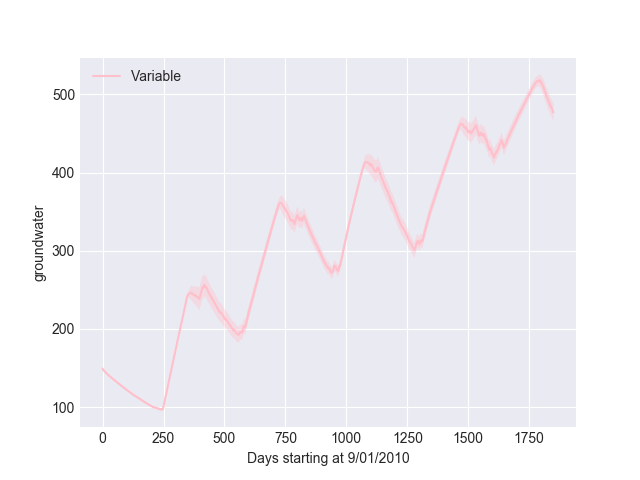
\includegraphics[width=.98\linewidth]{bad_gw}
  \captionof{figure}{Uniform groundwater}
  \label{fig:bad_gw}
\end{minipage}%
\begin{minipage}{.5\textwidth}
  \centering
  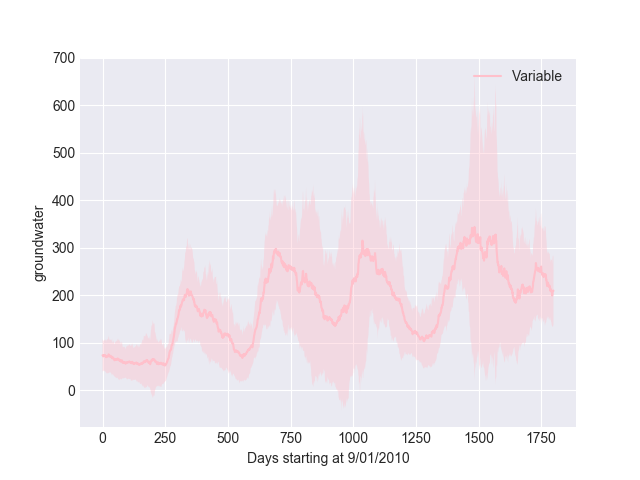
\includegraphics[width=.94\linewidth]{good_gw}
  \captionof{figure}{Perturbed groundwater}
  \label{fig:good_gw}
\end{minipage}
\end{figure}


\subsection{Continuous perturbation of streamflow and snow-water equivalent states}

Another method of smoothing the model's calibration process despite its over-reliance on groundwater was through the direct perturbation of streamflow and swe states. This perturbation guaranteed that ensemble collapse was never fully realized. Gaussian noise was added to the state vector $\mathbf{x^{i-}_{t}}$ before the parameter correction state and the state correction stage such that

\begin{equation}\label{eq:perturbation_str}
\mathbf{x^{i-}_{t,str}} + N(0,\mathbf{x^{i-}_{t,str}} \cdot -;pq_{str})
\end{equation}
and
\begin{equation}\label{eq:perturbation_swe}
\mathbf{x^{i-}_{t,swe}} + N(0,\mathbf{x^{i-}_{t,swe}} \cdot q_{swe})
\end{equation}

where $q_{str}$ and $q_{swe}$ are values between 0 and 1 representing model uncertainty. While the continuous perturation of streamflow and swe states was a useful debugging technique, large values for $q_{str}$ and $q_{swe}$ reduced the effectiveness of model calibration and were avoided.

\section{Small dataset}

To expedite the discovery of optimal initial values, errors, and minimum and maximum bounds for the complete dataset (see Table \ref{tab:t_param_min_max_initial} and table  \ref{tab:t_param_initial}) the small dataset was run and compared with the ranges proposed by \cite{Seibert1997} and \cite{Wallner2013} and then run again with boundaries optimized for the current model.  The small dataset, which was comprised of 3 catchments around the Biterroot valley and consisted of one gauged catchment (henceforth referred to as catchment 241) and 2 ungauged catchments (catchments 244 and 248), was run over a period of 1095 days starting a little before Fall of 2010. Simulations began in September so modeled snowfall accumulation could be corrected first, allowing accurate snow melts to inform streamflow runoff in the Spring and Summer. All parameters in the small dataset converged to a set of values quickly but quickly readjusted when significant differences arose between the observed and modeled states.

%The state, groundwater, and parameter results from the small dataset runs may be seen in figures \ref{fig:str_state_small}, \ref{fig:str_innovation_small}, \ref{fig:swe \ref{fig:swe_innovation_small} \ref{fig:str_params_small}, \ref

\subsection{Streamflow states and parameters}

\begin{figure}
\centering
\begin{minipage}{.33\textwidth}
  \centering
  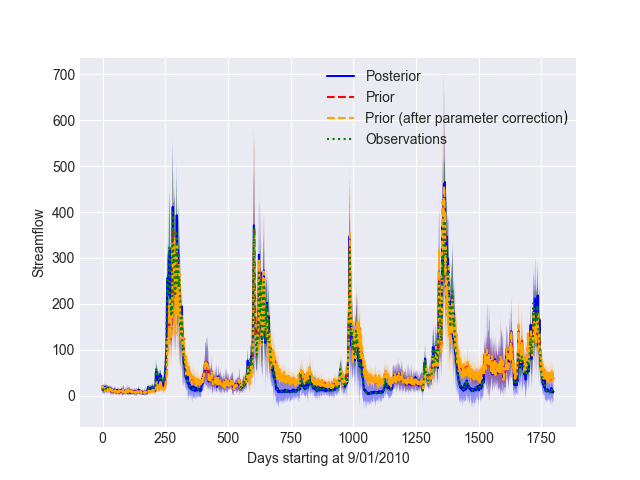
\includegraphics[width=.98\linewidth]{smallds_str_state_241}
  \label{fig:241st}
\end{minipage}%
\begin{minipage}{.33\textwidth}
  \centering
  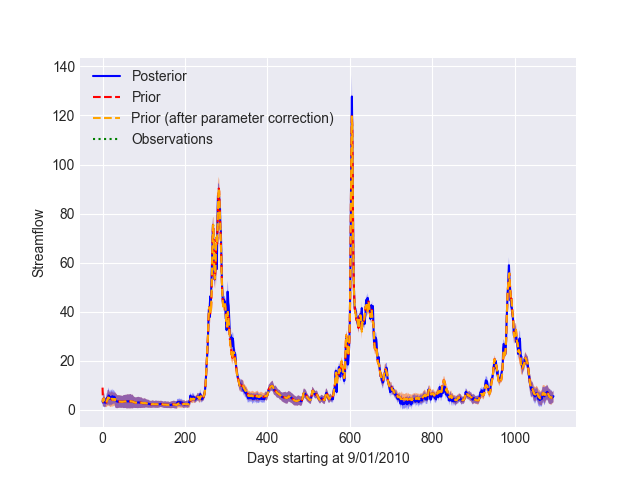
\includegraphics[width=.98\linewidth]{smallds_str_state_244}
  \label{fig:244st}
\end{minipage}
\begin{minipage}{.33\textwidth}
  \centering
  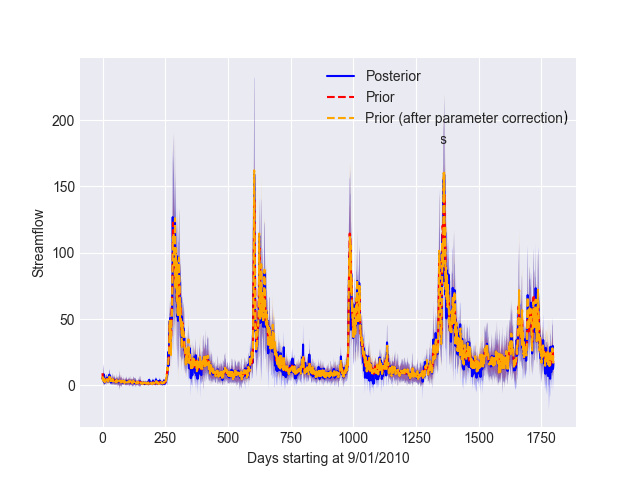
\includegraphics[width=.98\linewidth]{smallds_str_state_248}
  \label{fig:248st}
\end{minipage}
\captionof{figure}{Streamflow states for the 3 small dataset catchments. From left to right: 241,244,248}
\label{fig:str_state_small}
\end{figure}

The gaged catchment 241's posterior streamflow state (leftmost graph in Figure \ref{fig:str_state_small}) snapped to the observations quickly. Catchment 241's post-parameter corrected streamflow values (shown in yellow on the figures in \ref{fig:str_state_small}) also closely followed the observations. Notice the slight discrepancy between the post parameter correction state and posterior state seen in the first graph in Figure \ref{fig:str_state_small} during the Winter time periods. While state correction continuously tried to move streamflow down to a match the observed Winter state, parameters were not found that allowed streamflow to perfectly match the observed states. This behavior is connected to the value of the lower groundwater reservoir and is seen to some degree in the Winter months in almost all streamflow state graphs.

The lower groundwater reservoir in all three catchments  rose 20mm-200mm throughout the 1095 day filtering period (Figure \ref{fig:gw_small}). Throughout this time the filter's values for \texttt{ck2} and \texttt{perc}, two parameters that impact the buildup and dispersion of lower groundwater, remained unchanged. The stabilization of the lower groundwater component in the hydrologic model is explored in Chapter 5.

\begin{figure}
\centering
\begin{minipage}{.33\textwidth}
  \centering
  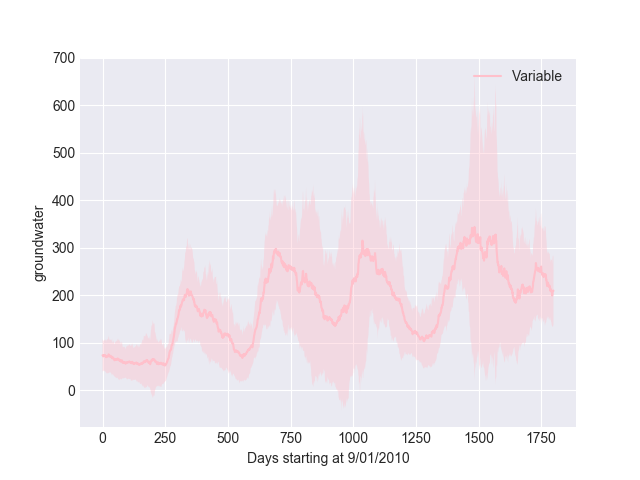
\includegraphics[width=.98\linewidth]{smallds_gw_state_241}
  \label{fig:241gw}
\end{minipage}%
\begin{minipage}{.33\textwidth}
  \centering
  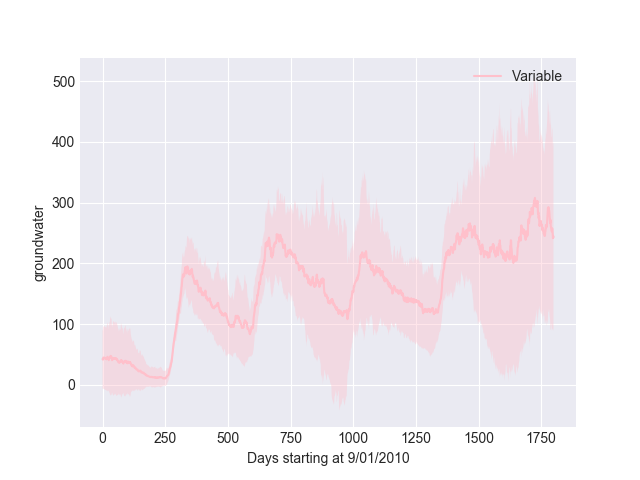
\includegraphics[width=.98\linewidth]{smallds_gw_state_244}
  \label{fig:244gw}
\end{minipage}
\begin{minipage}{.33\textwidth}
  \centering
  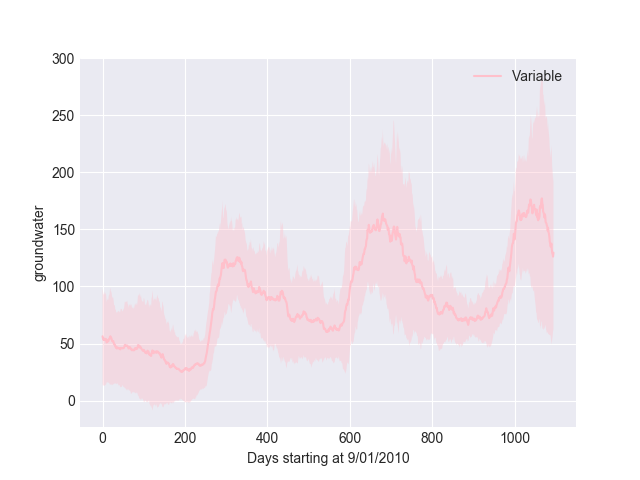
\includegraphics[width=.98\linewidth]{smallds_gw_state_248}
  \label{fig:248gw}
\end{minipage}
\captionof{figure}{Groundwaters for the 3 catchments}
\label{fig:gw_small}
\end{figure}

As seen in the plots in Figure \ref{fig:cks_small}, parameter ensembles converged to the ensemble mean within the first 5-10 days and remained stable until the Spring and Summer months. When modeled results deviated significantly from observed states the ensembles reconstituted and searched for a more optimal value. This stair-stepping behavior is linked to the new hierarchical parameter perturbation algorithms and appears to be standard behavior for the DSHEnKF algorithm. The implications of this are explored in Chapter 5. Importantly, all catchment values remained unique and did not coverage to a spatial mean.

\begin{figure}[h]
    \centering
    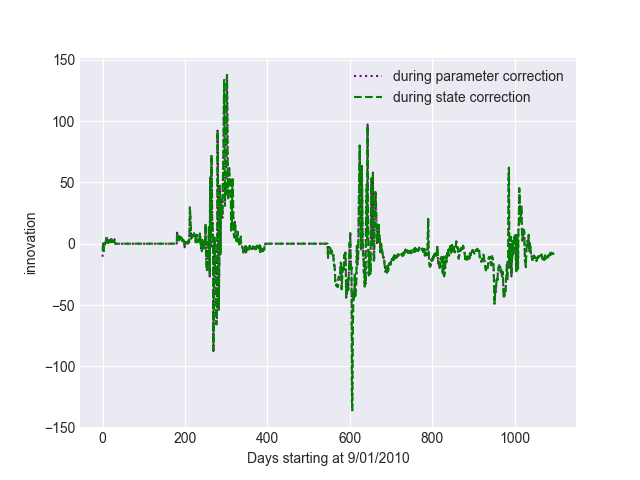
\includegraphics[width=0.5\textwidth]{str_innovation_small}
    \caption{Streamflow innovation (catchment 241)}
    \label{fig:str_innovation_small}
\end{figure}


\begin{figure}
\begin{tabular}{ccc}

\subcaptionbox{241:\texttt{ck0}\label{2}}{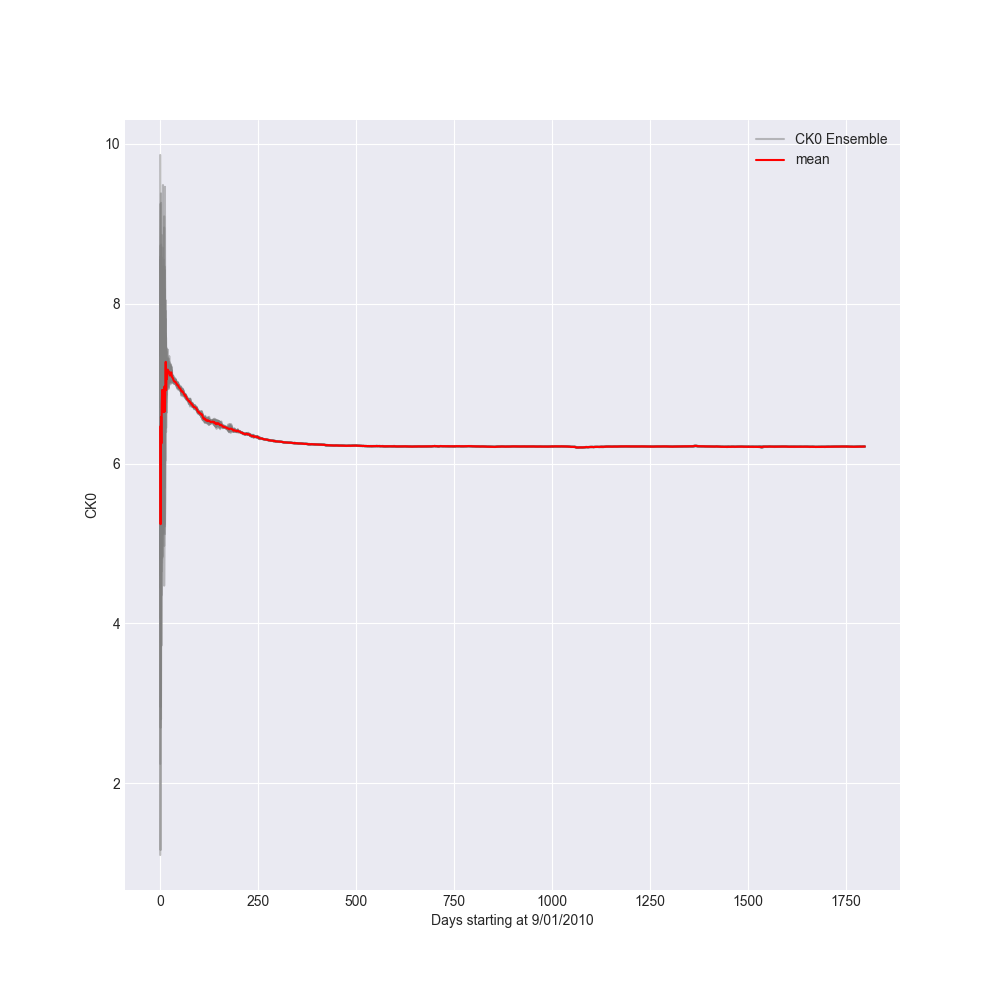
\includegraphics[width = .33\linewidth]{smallds_ck0_241}} &
\subcaptionbox{241:\texttt{ck1}\label{1}}{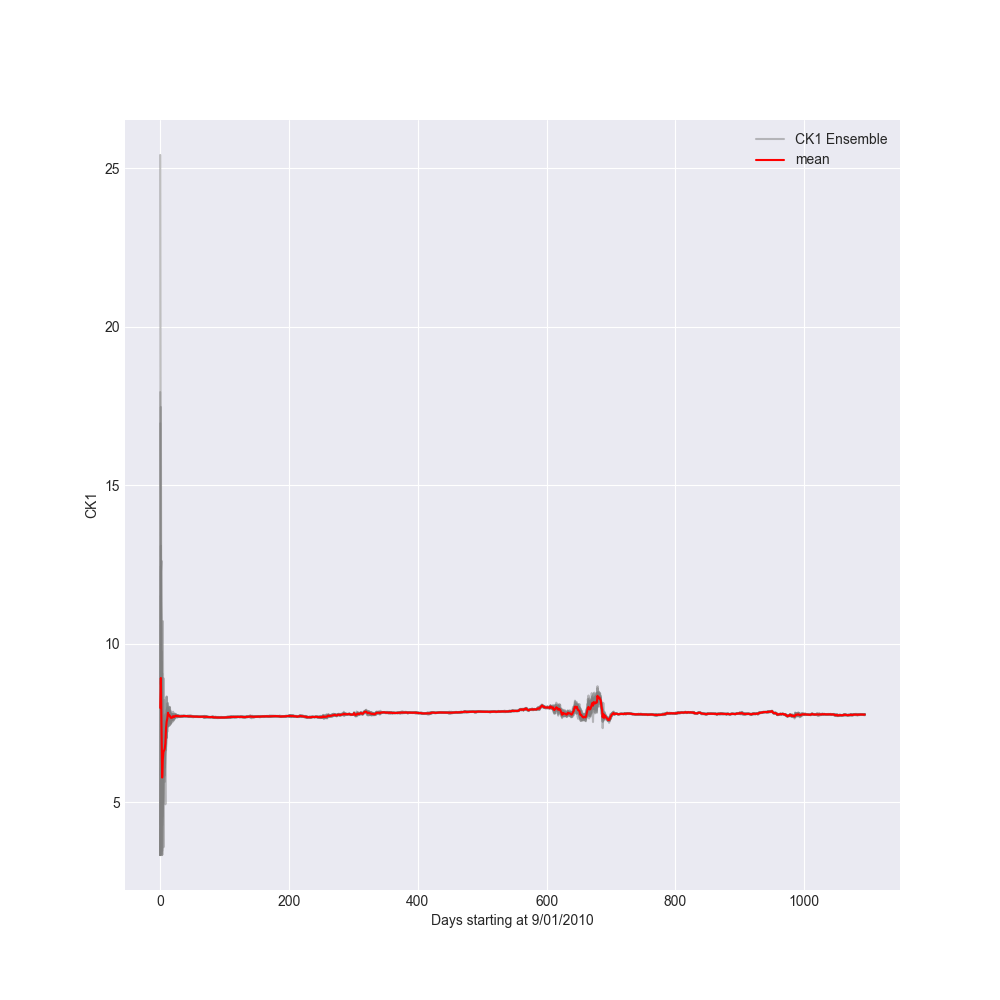
\includegraphics[width = .33\linewidth]{smallds_ck1_241}} &
\subcaptionbox{241:\texttt{ck2}\label{2}}{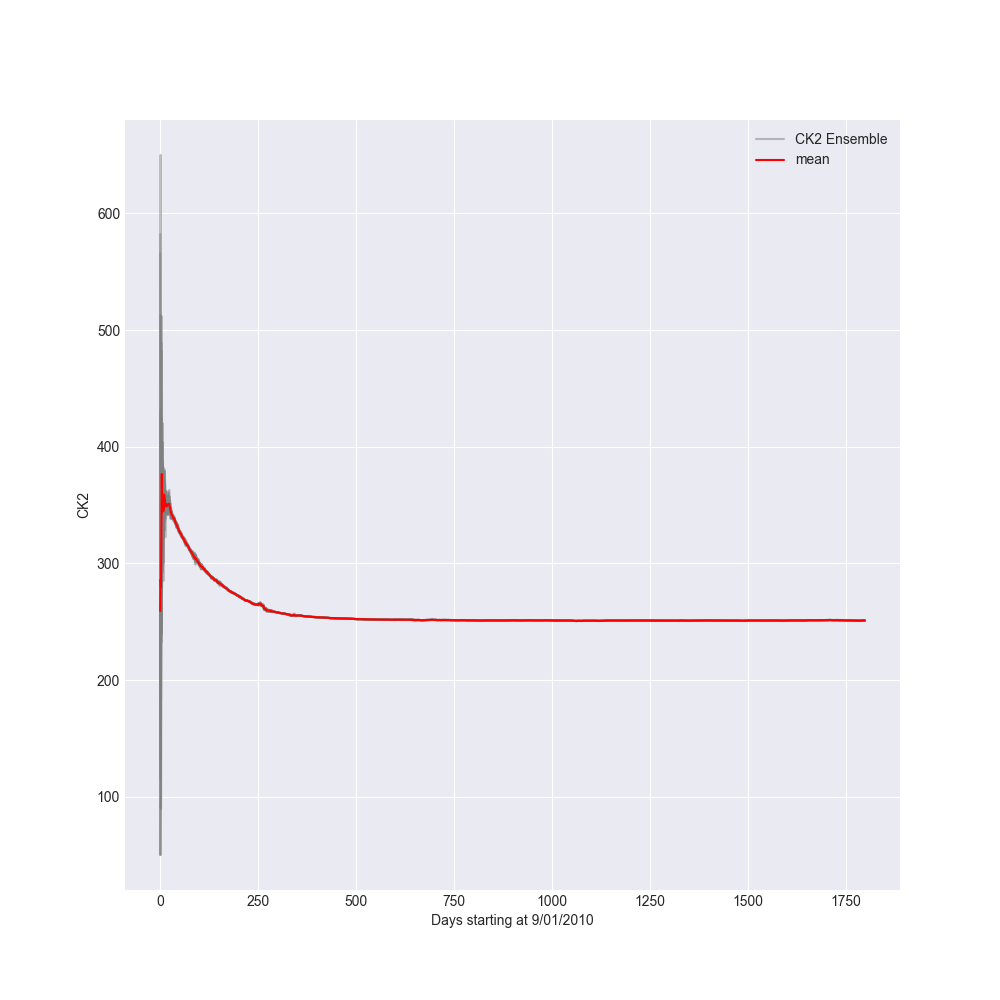
\includegraphics[width = .33\linewidth]{smallds_ck2_241}}\\
\subcaptionbox{244:\texttt{ck0}\label{2}}{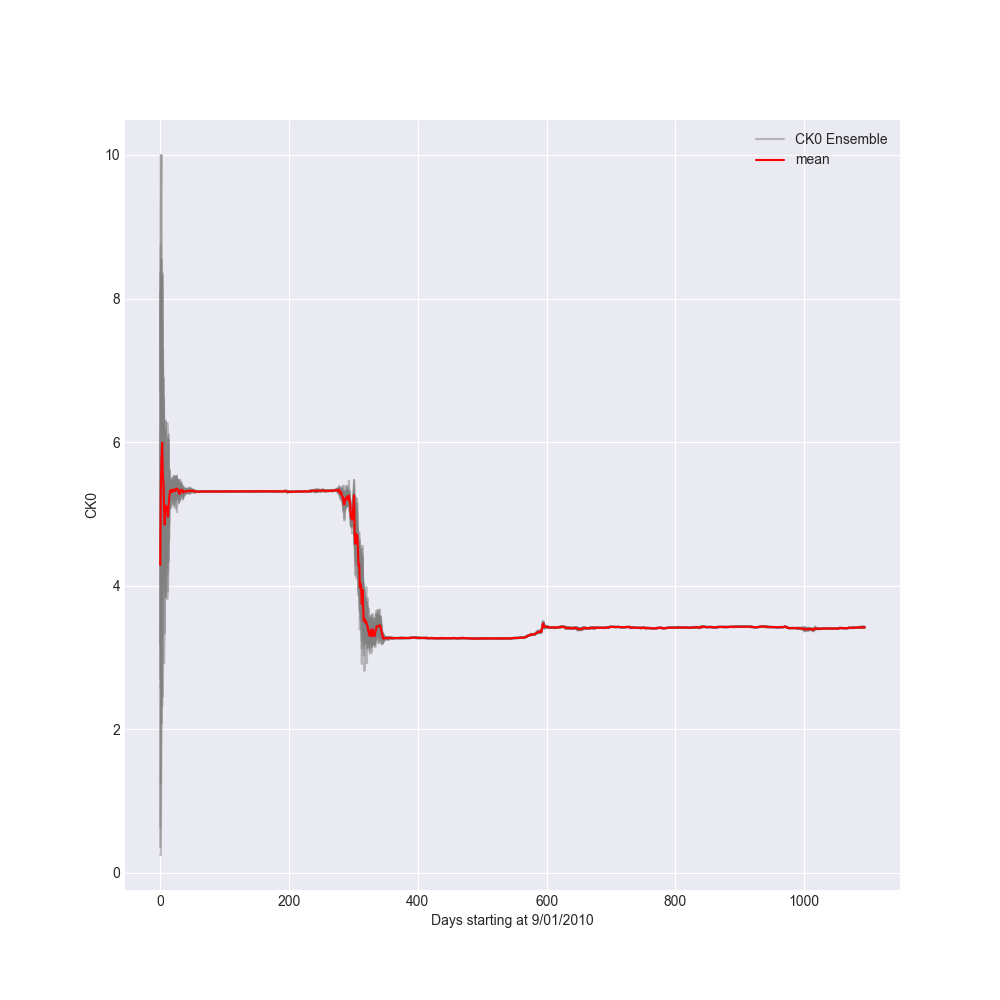
\includegraphics[width = .33\linewidth]{smallds_ck0_244}} &
\subcaptionbox{244:\texttt{ck1}\label{1}}{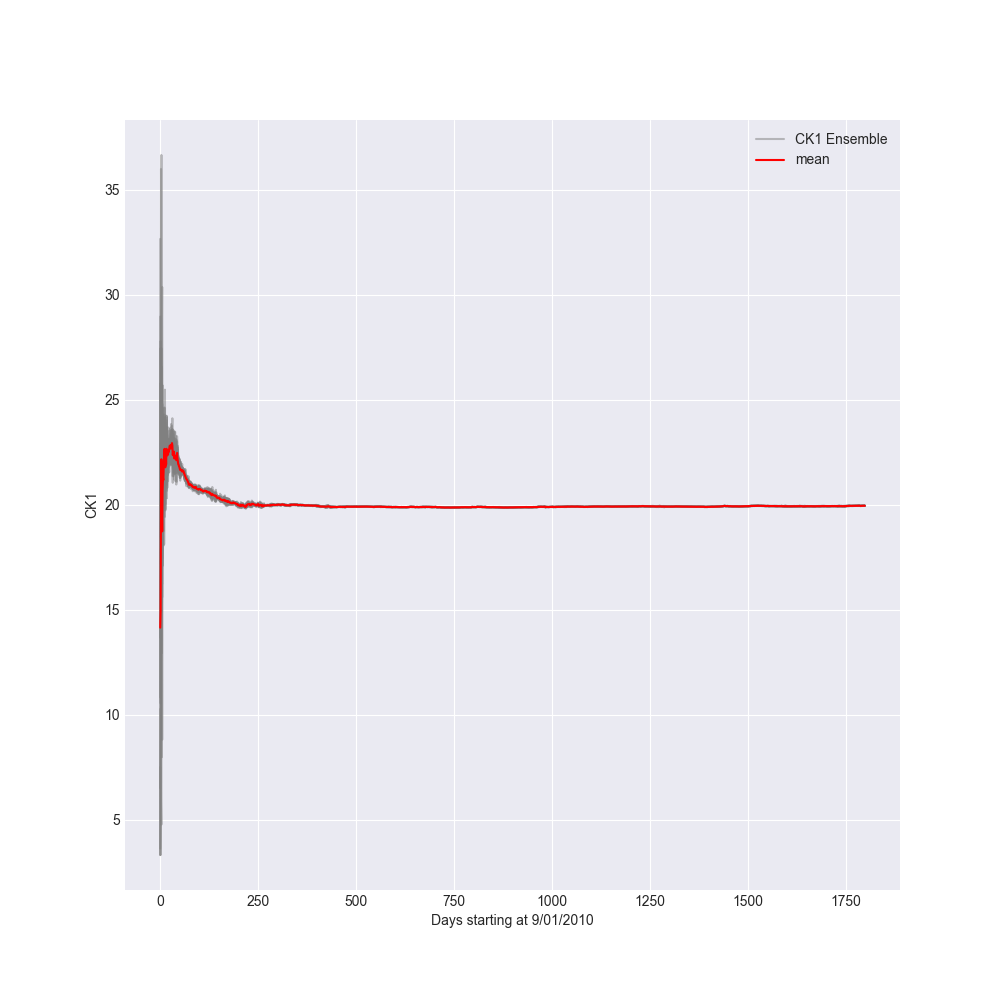
\includegraphics[width = .33\linewidth]{smallds_ck1_244}} &
\subcaptionbox{244:\texttt{ck2}\label{2}}{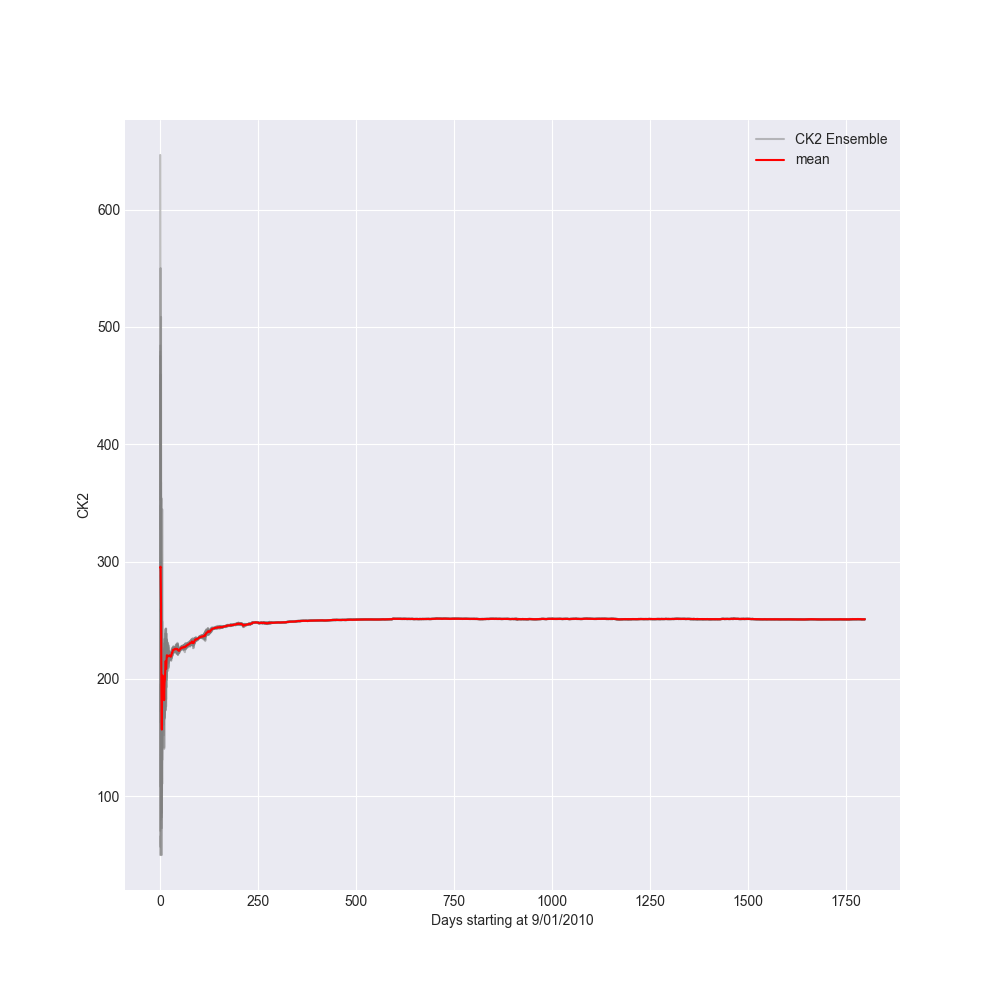
\includegraphics[width = .33\linewidth]{smallds_ck2_244}}\\
\subcaptionbox{248:\texttt{ck0}\label{2}}{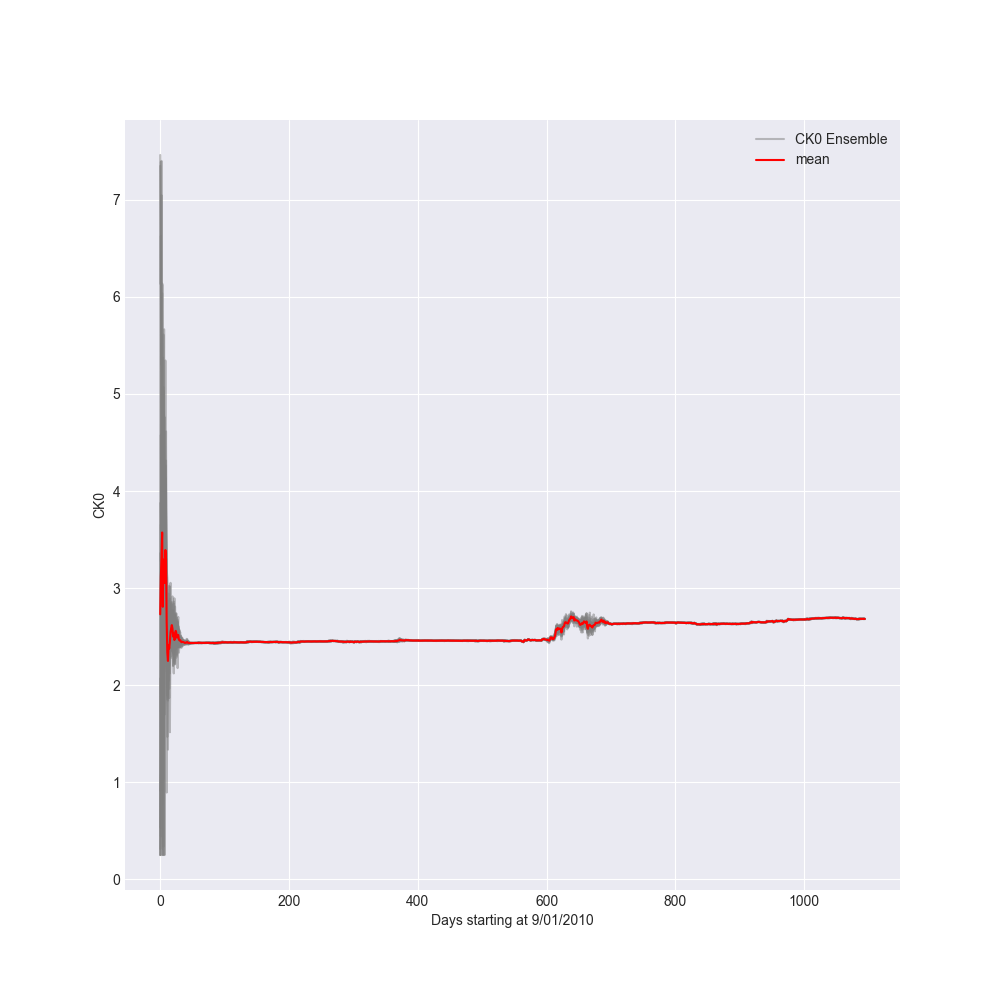
\includegraphics[width = .33\linewidth]{smallds_ck0_248}} &
\subcaptionbox{248:\texttt{ck1}\label{1}}{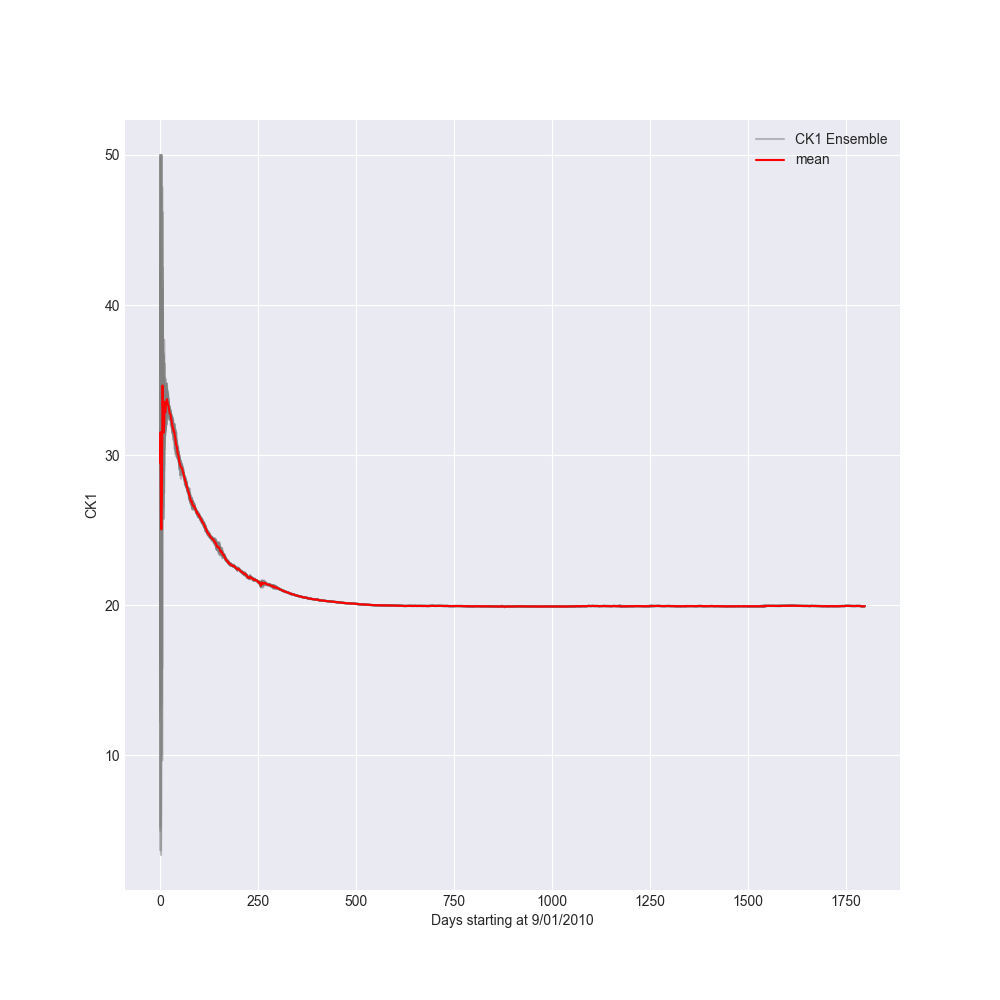
\includegraphics[width = .33\linewidth]{smallds_ck1_248}} &
\subcaptionbox{248:\texttt{ck2}\label{2}}{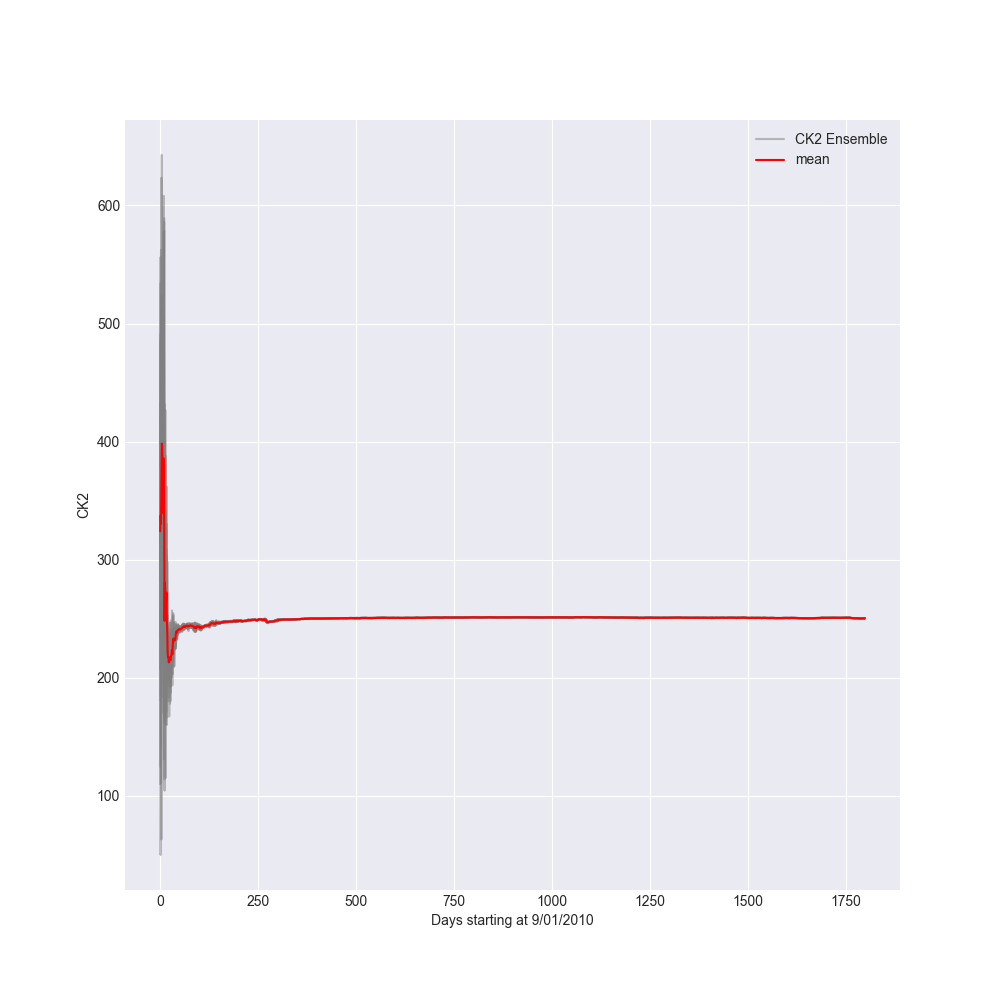
\includegraphics[width = .33\linewidth]{smallds_ck2_248}}

\end{tabular}
\captionof{figure}{Convergence of \texttt{ck} parameters for all 3 catchments}
\label{fig:cks_small}
\end{figure}

\begin{table}[]
\caption{Hyperparameters - parameter perturbations and min/max ranges} 
\begin{tabular}{llll}
Parameter ($\theta$) & $q$ & Min & Max \\ \hline
Degree Day Factor (\texttt{ddf})                 & .75mm$^\circ$C$^{-1}$d$^{-1}$ & 1mm$^\circ$C$^{-1}$d$^{-1}$ & 8mm$^\circ$C$^{-1}$d$^{-1}$ \\
Tempature Threshold (\texttt{thres})                & .5$^\circ$C & -2.5$^\circ$C & 2.5$^\circ$C \\
Potential Evapo-Transpiration (\texttt{aet\_lp})              & .15 & .3 & 1\\
Ponded water to soil storage (\texttt{soil\_beta})          & 1.75 & 1 & 6 \\
Soil compartment max capacity (\texttt{soil\_max\_wat})       & 40 & 50mm & 500mm \\
Immediate runoff (\texttt{ck0})       & 6d$^{-1}$ & .25d$^{-1}$ & 10d$^{-1}$ \\
Fast runoff (\texttt{ck1})      & 25d$^{-1}$ & 3.33d$^{-1}$ & 50d$^{-1}$\\
Groundwater runoff (\texttt{ck2})       & 350d$^{-1}$ & 50d$^{-1}$ & 650d$^{-1}$ \\
Groundwater water storage threshold (\texttt{hl1})       & 25mm & 0mm & 50mm \\
Groundwater peculation (\texttt{perc})       & 1.5d & 3d & 50d \\
%Wave celerity (\texttt{K})         & 82400 & 81576 & 84872 \\
Wave dispersion (\texttt{e})       & .35 & .25 & .4 \\
\end{tabular}
\label{tab:t_param_min_max_initial}
\end{table}

\begin{table}[]
\caption{Initial parameter values} 
\begin{tabular}{ll}
Parameter ($\theta$) & Starting Value \\ \hline
Degree Day Factor (\texttt{ddf})                 & .4mm$^\circ$C$^{-1}$d$^{-1}$ \\
Tempature Threshold (\texttt{thres})                & 2$^\circ$C \\
Potential Evapo-Transpiration (\texttt{aet\_lp})              & .5\\
Ponded water to soil storage (\texttt{soil\_beta})          & 4.8 \\
Soil compartment max capacity (\texttt{soil\_max\_wat})       & 400mm \\
Immediate runoff (\texttt{ck0})       & 20d$^{-1}$ \\
Fast runoff (\texttt{ck1})      & 200d$^{-1}$ \\
Groundwater runoff (\texttt{ck2})       & 300d$^{-1}$ \\
Groundwater water storage threshold (\texttt{hl1})       & 20mm \\
Groundwater peculation (\texttt{perc})       & 10d \\
Wave dispersion (\texttt{e})       & .37 \\
\end{tabular}
\label{tab:t_param_initial}
\end{table}

\subsection{Snow-water equivalent states and parameters}

\begin{figure}
\centering
\begin{minipage}{.33\textwidth}
  \centering
  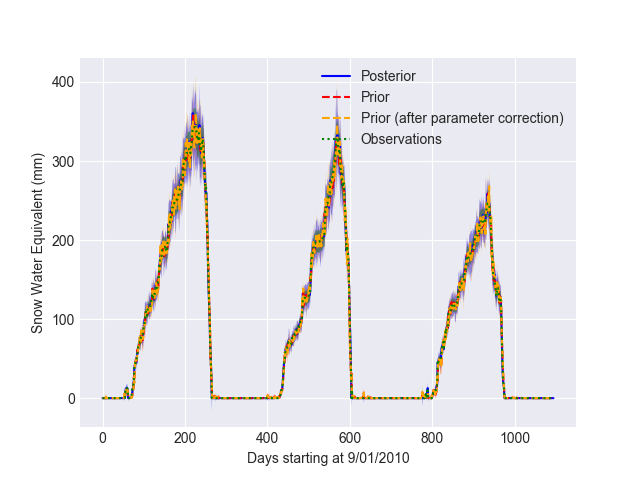
\includegraphics[width=.98\linewidth]{smallds_swe_state_241}
  \label{fig:241swe}
\end{minipage}%
\begin{minipage}{.33\textwidth}
  \centering
  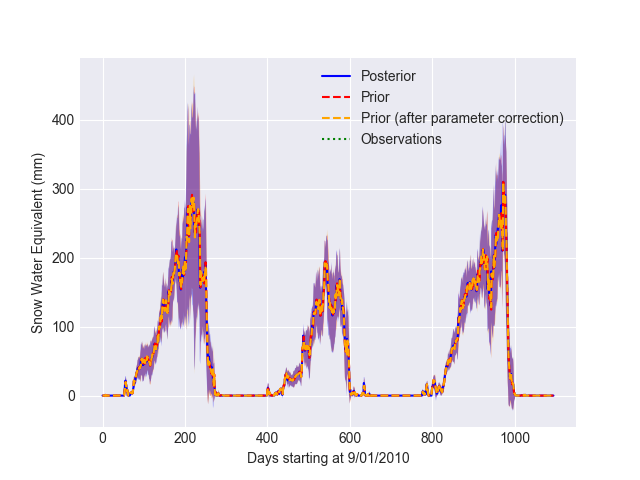
\includegraphics[width=.98\linewidth]{smallds_swe_state_244}
  \label{fig:244swe}
\end{minipage}
\begin{minipage}{.33\textwidth}
  \centering
  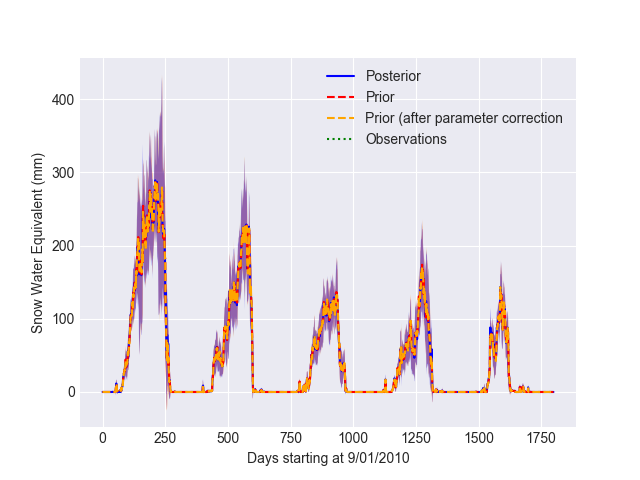
\includegraphics[width=.98\linewidth]{smallds_swe_state_248}
  \label{fig:248swe}
\end{minipage}
\captionof{figure}{Snow-water equivalent states for the 3 catchments. From left to right: 241, 244, 248}
\label{fig:swe_state_small}
\end{figure}


\begin{figure}[h]
    \centering
    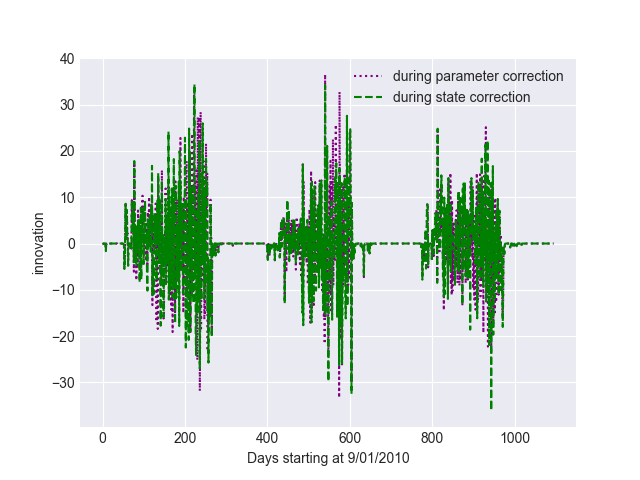
\includegraphics[width=0.5\textwidth]{swe_innovation_small}
    \caption{SWE innovation (catchment 241)}
    \label{fig:swe_innovation_small}
\end{figure}

Snow-water equivalent states and parameters behaved similarly to their streamflow counterparts. Catchment 241's snow-water equivalent states (Figure \ref{fig:swe_state_small}) snapped to the observations quickly. Snow-water equivalent innovation (Figure \ref{fig:swe_innovation_small}) is somewhat less biased then streamflow innovation (Figure \ref{fig:str_innovation_small}). Snow-water equivalent parameters behaved similarly to their streamflow counterparts. All ensembles and catchments converged to ensemble means within the first 20 days and did not significantly deviate from their chosen values throughout the remainder of calibration (Figure \ref{fig:swe_params_small}.) Similarly to the streamflow parameter ensembles, each catchment's value remained unique and did not converge to the mean (more easily seen in Figure \ref{fig:swe_params_small_full}.)



\begin{figure}
\begin{tabular}{cc}

\subcaptionbox{241:\texttt{ddf}\label{2}}{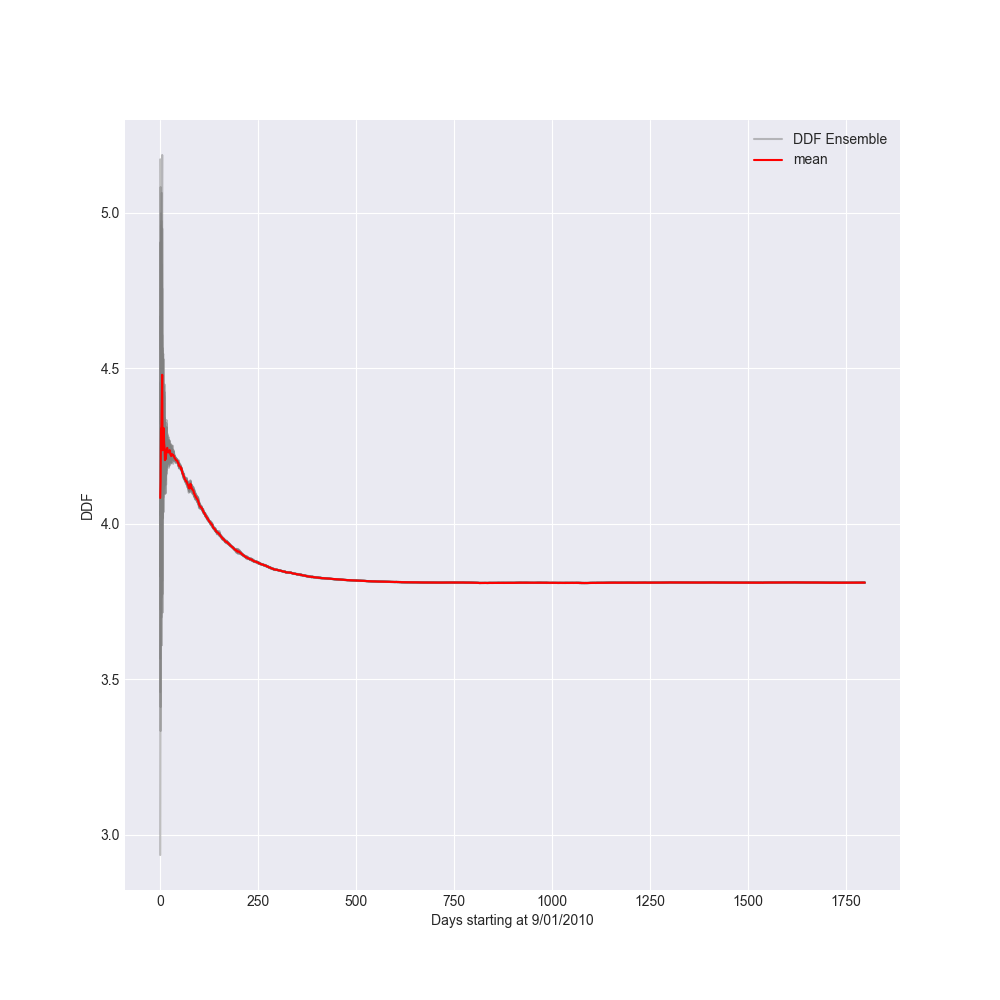
\includegraphics[width = .48\linewidth]{smallds_ddf_241}} &
\subcaptionbox{241:\texttt{thres}\label{2}}{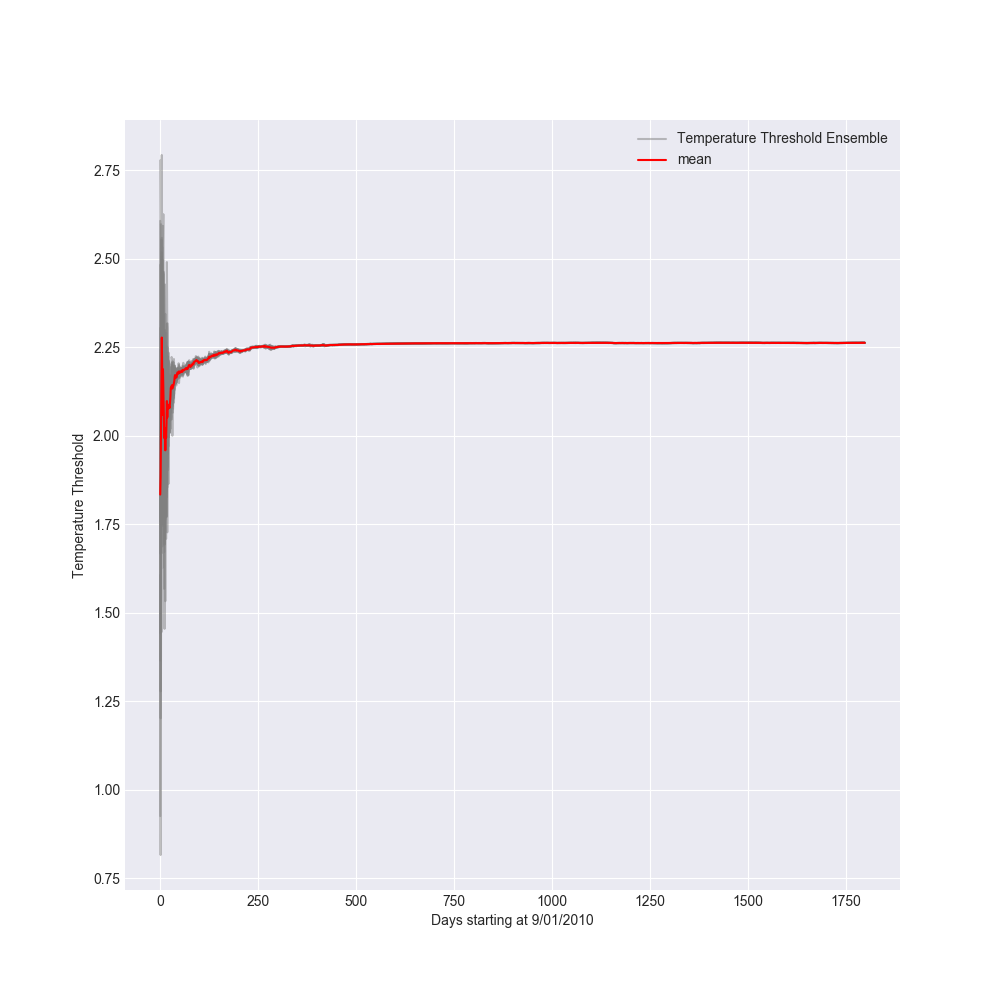
\includegraphics[width = .48\linewidth]{smallds_pp_241}}\\
\subcaptionbox{244:\texttt{ddf}\label{2}}{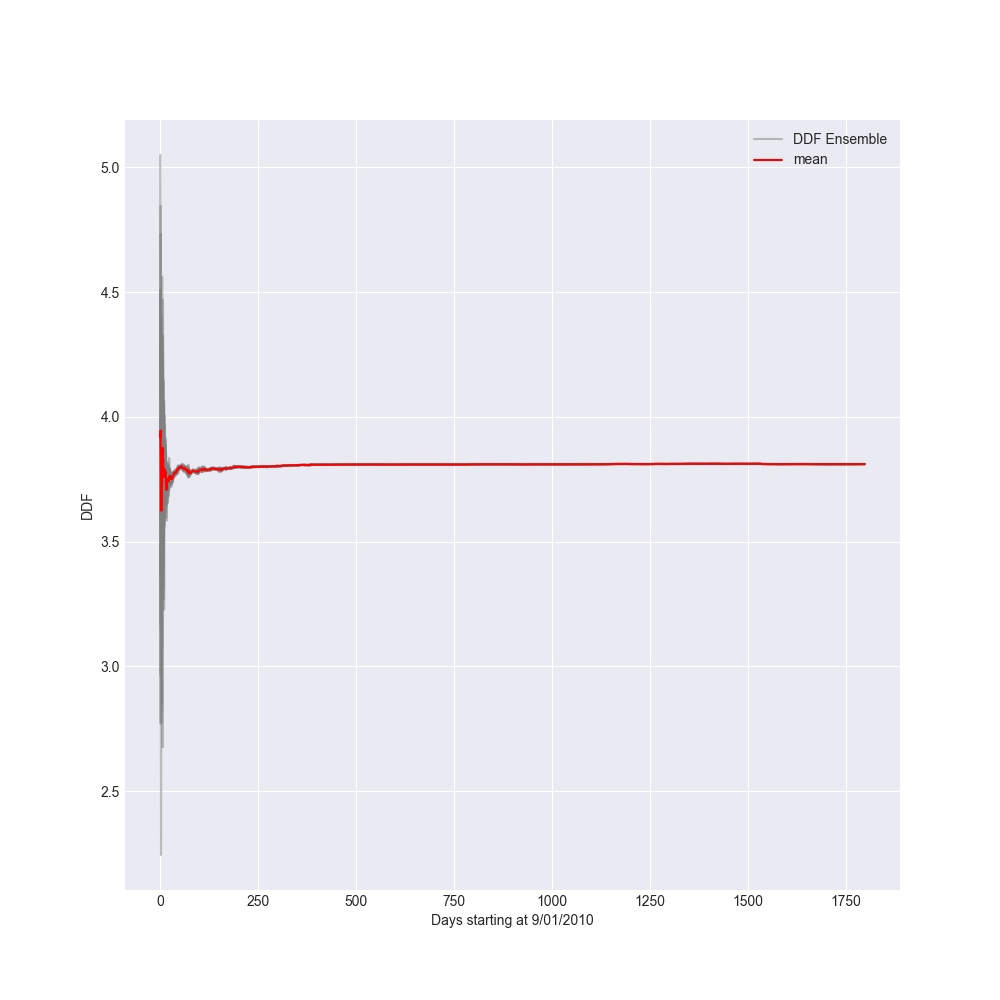
\includegraphics[width = .48\linewidth]{smallds_ddf_244}} &
\subcaptionbox{244:\texttt{thres}\label{2}}{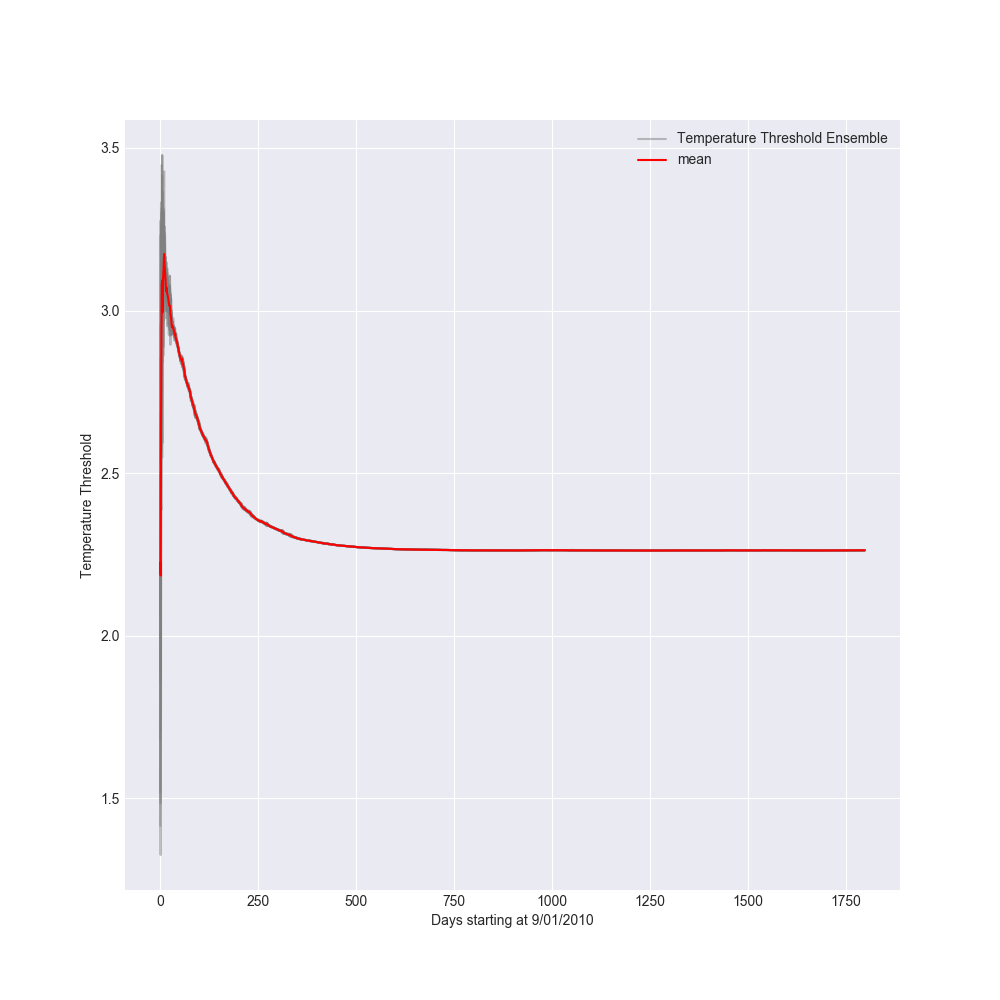
\includegraphics[width = .48\linewidth]{smallds_pp_244}}\\
\subcaptionbox{248:\texttt{ddf}\label{2}}{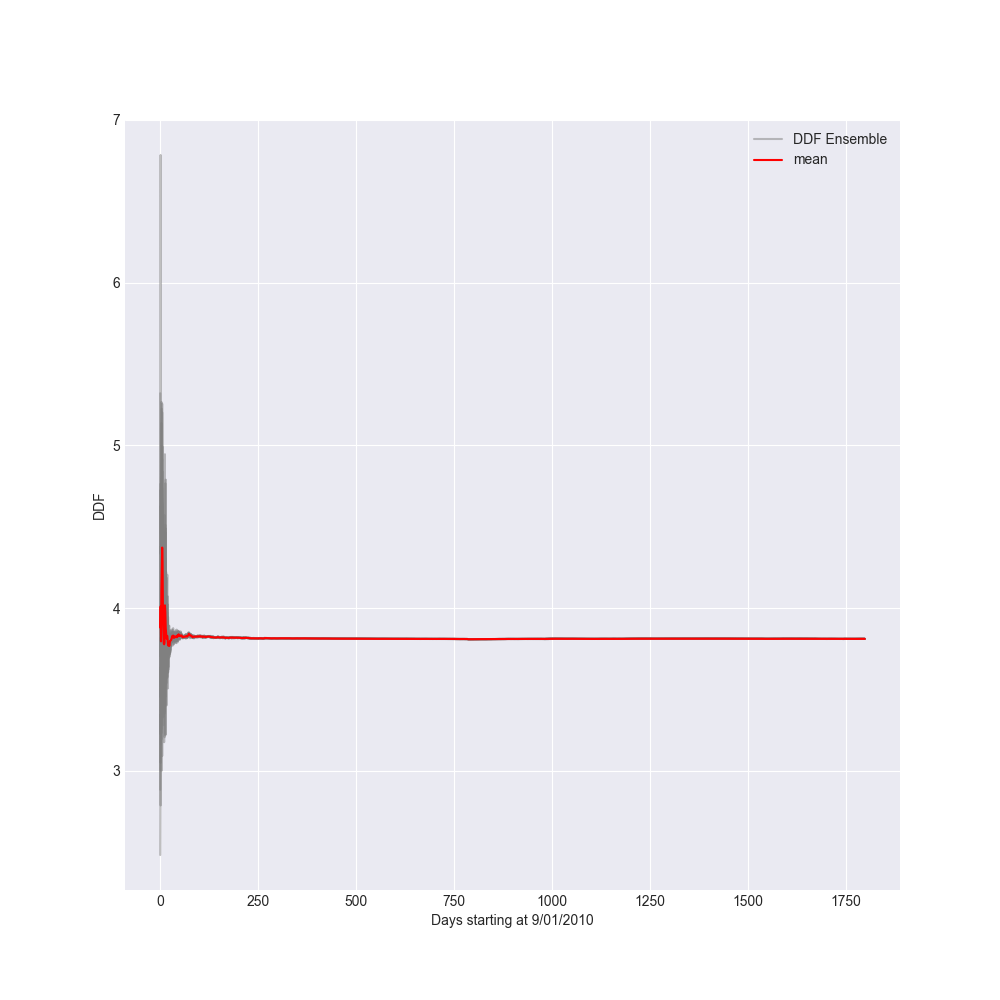
\includegraphics[width = .48\linewidth]{smallds_ddf_248}} &
\subcaptionbox{248:\texttt{thres}\label{1}}{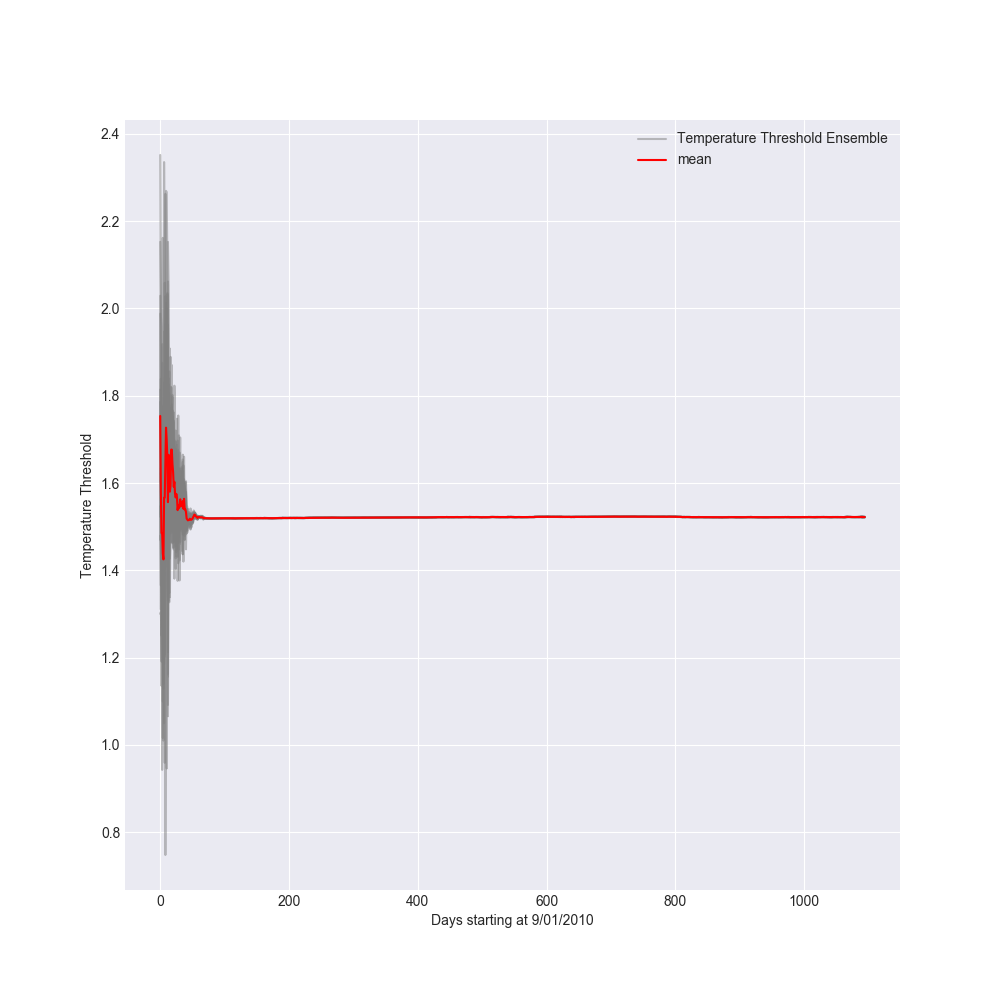
\includegraphics[width = .48\linewidth]{smallds_pp_248}}

\end{tabular}
\captionof{figure}{Convergence of \texttt{ddf} and \texttt{thres} parameters for all 3 catchments}
\label{fig:swe_params_small}
\end{figure}

\begin{figure}
\begin{tabular}{cc}

\subcaptionbox{All catchments:\texttt{ddf}\label{group17swe_ddf_small}}{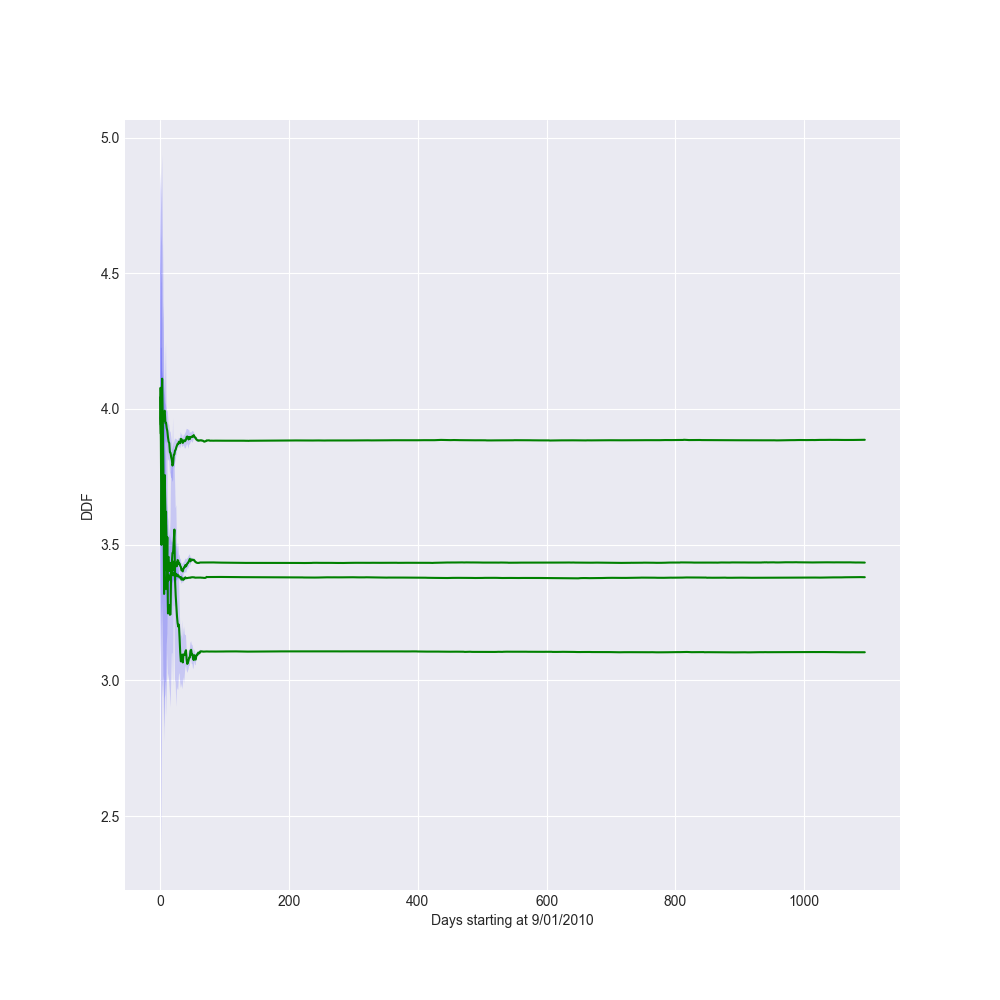
\includegraphics[width = .48\linewidth]{group17swe_ddf_small}} &
\subcaptionbox{All catchments:\texttt{pp}\label{group17swe_pp_small}}{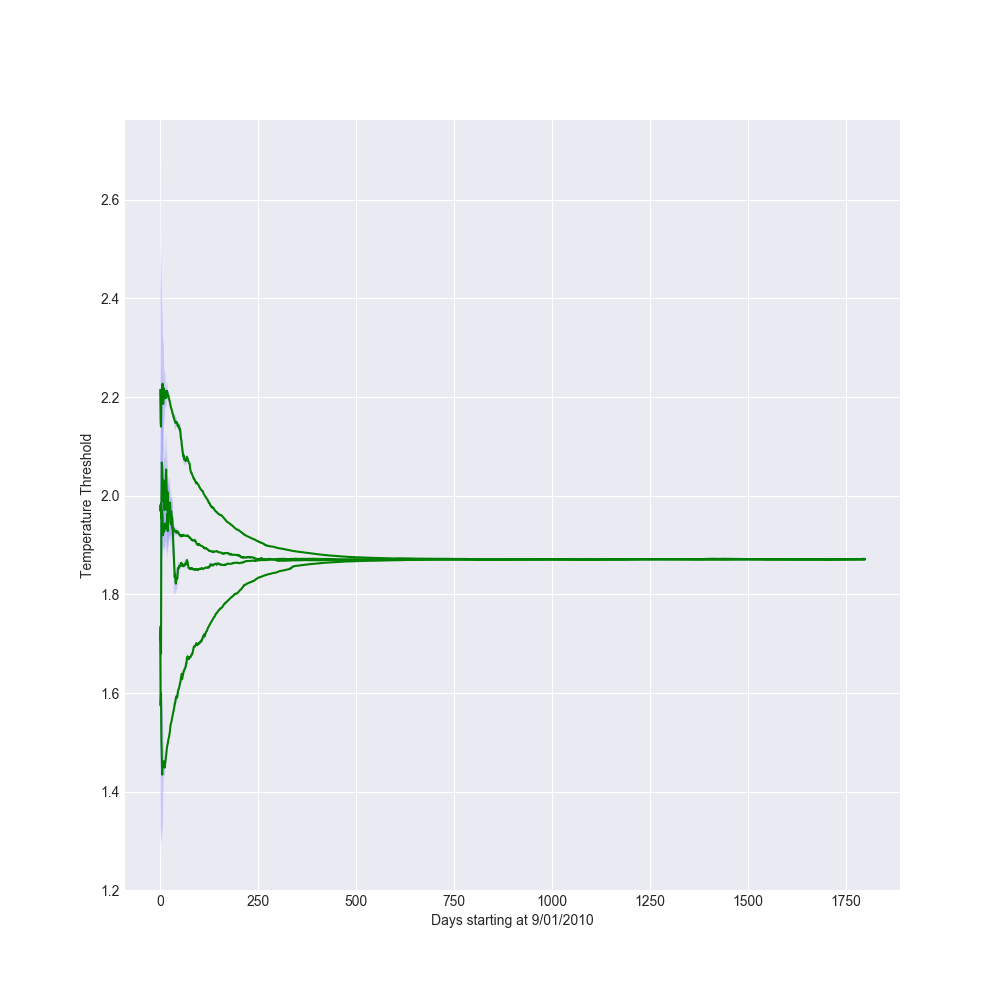
\includegraphics[width = .48\linewidth]{group17swe_pp_small}}
\end{tabular}
\captionof{figure}{All SWE parameters stabilized quickly during the run of the small dataset. \texttt{a}  = .9}
\label{fig:swe_params_small_full}
\end{figure}

\pagebreak

\section{Complete Dataset}

After workable initial values, errors, and boundaries and had been selected the complete dataset was calibrated. Calibration of the complete dataset was computationally expensive and a balance had to be struck between ensemble size, time run, and data collected per timestep. For these results a full three years (1095 days) was run with 100 ensemble members. The effects of different ensemble sizes on results is discussed in Chapter 5. Running the DSHEnKF on the large dataset produced good results that point to both strengths in the hierarchical design and further research opportunities.

\subsection{Streamflow states and parameters}

Streamflow calibration on the complete dataset progressed in a similar way to calibration on the small dataset, but more variation in geographic location helped identify patterns in the DSHEnKF method. All parameters in individual watersheds collapsed to their means in the first 30 days and reconstituted when large discrepancies existed between modeled behavior and observed streamflow behavior. While gauged posterior states matched their observations, innovation tended to be biased in either the positive or the negative direction (Figure \ref{fig:str_state_296}.) It is believed that this is primarily due to the model's heavy dependence on groundwater to influence a timestep's state as discussed in section \autoref{sec:perturbation_of_states}.

Streamflow parameters converged in a similar fashion to the small dataset's parameters (Figure \ref{fig:str_params_cks}.) Note how the ensembles tend to reconstitute during the Spring and Summer time periods - this is most noticeable in the \texttt{ck0} graph in \ref{fig:str_params_198}. Patterns in the distribution of streamflow parameters are explored in Chapter 5.

\begin{figure}
\centering
\begin{minipage}{.48\textwidth}
  \centering
  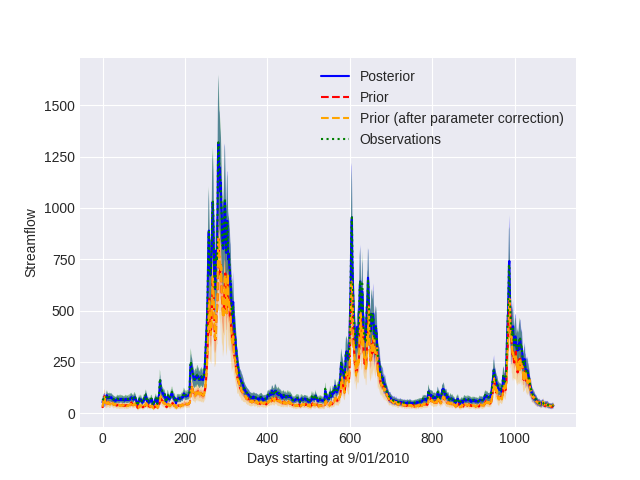
\includegraphics[width=.98\linewidth]{ds_str_state_198}
  \label{fig:296str}
\end{minipage}%
\begin{minipage}{.48\textwidth}
  \centering
  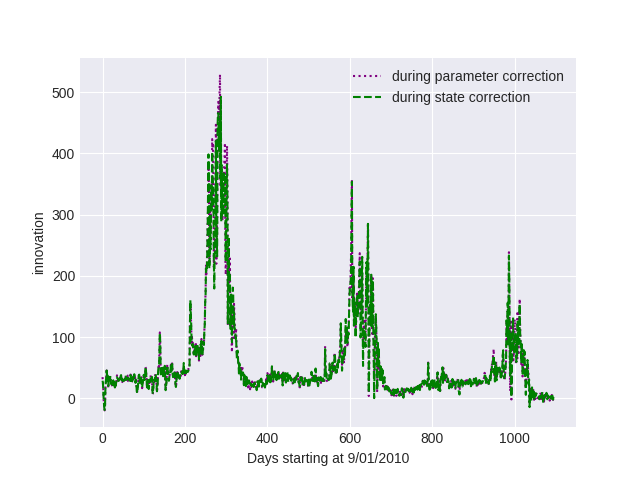
\includegraphics[width=.98\linewidth]{ds_str_state_198_innovation}
  \label{fig:296strinnovation}
\end{minipage}
\captionof{figure}{A gauged streamflow state (catchment 198)  and its innovation}
\label{fig:str_state_296}
\end{figure}

\begin{figure}
\begin{tabular}{cc}

\subcaptionbox{\texttt{ck0}\label{2}}{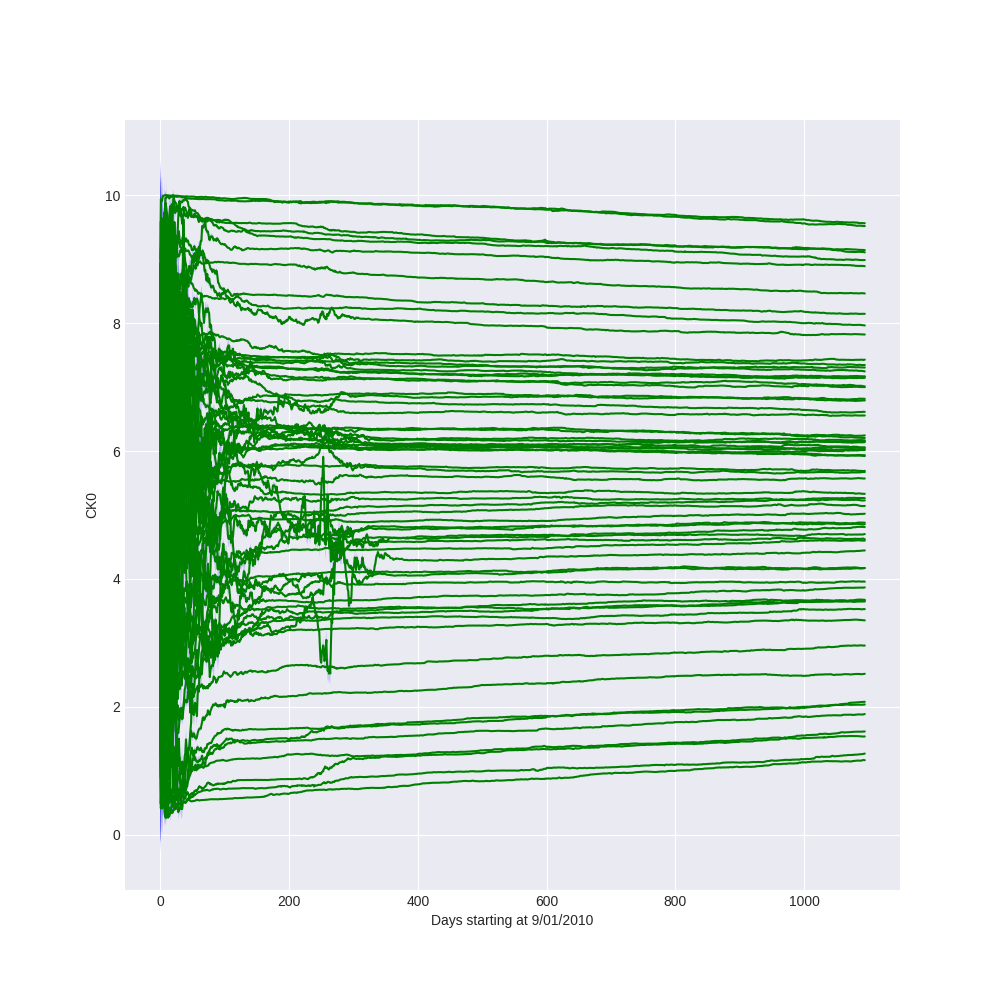
\includegraphics[width = .48\linewidth]{group17streamflow_ck0}} &
\subcaptionbox{\texttt{ck1}\label{2}}{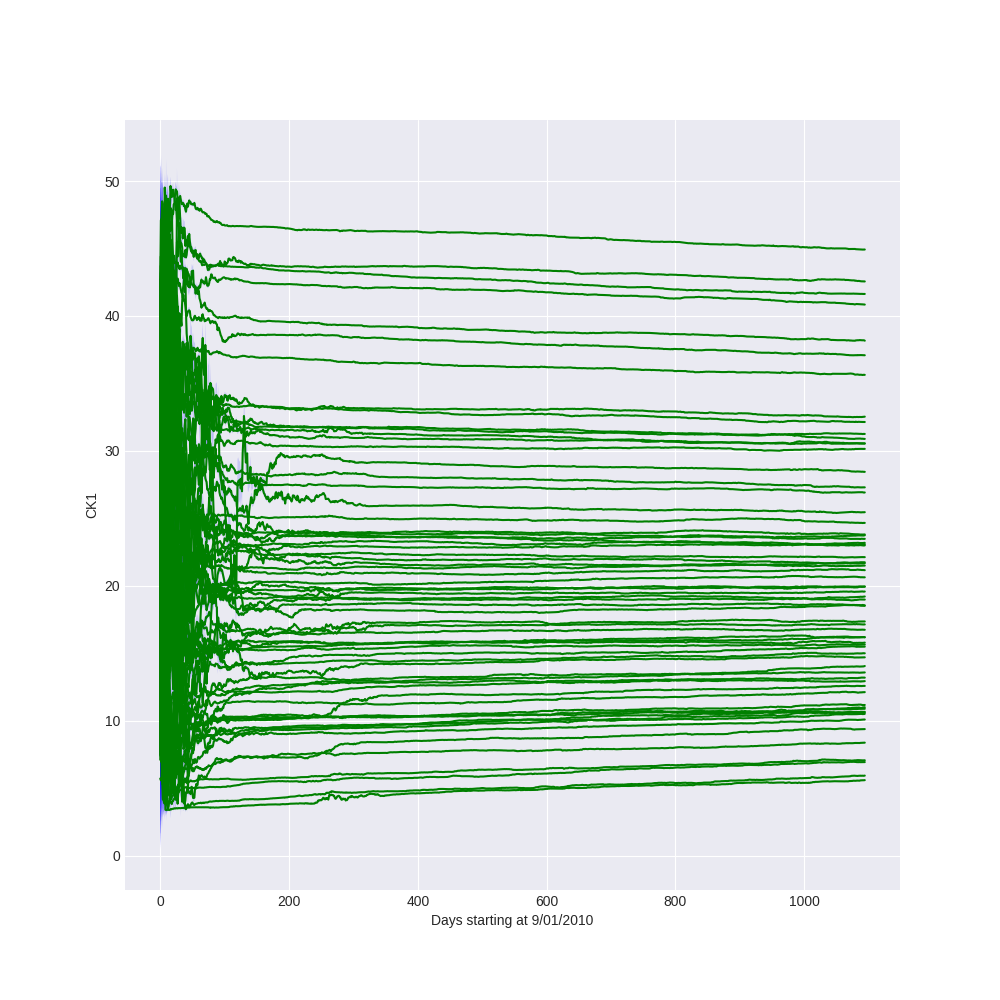
\includegraphics[width = .48\linewidth]{group17streamflow_ck1}}\\
\subcaptionbox{\texttt{ck2}\label{2}}{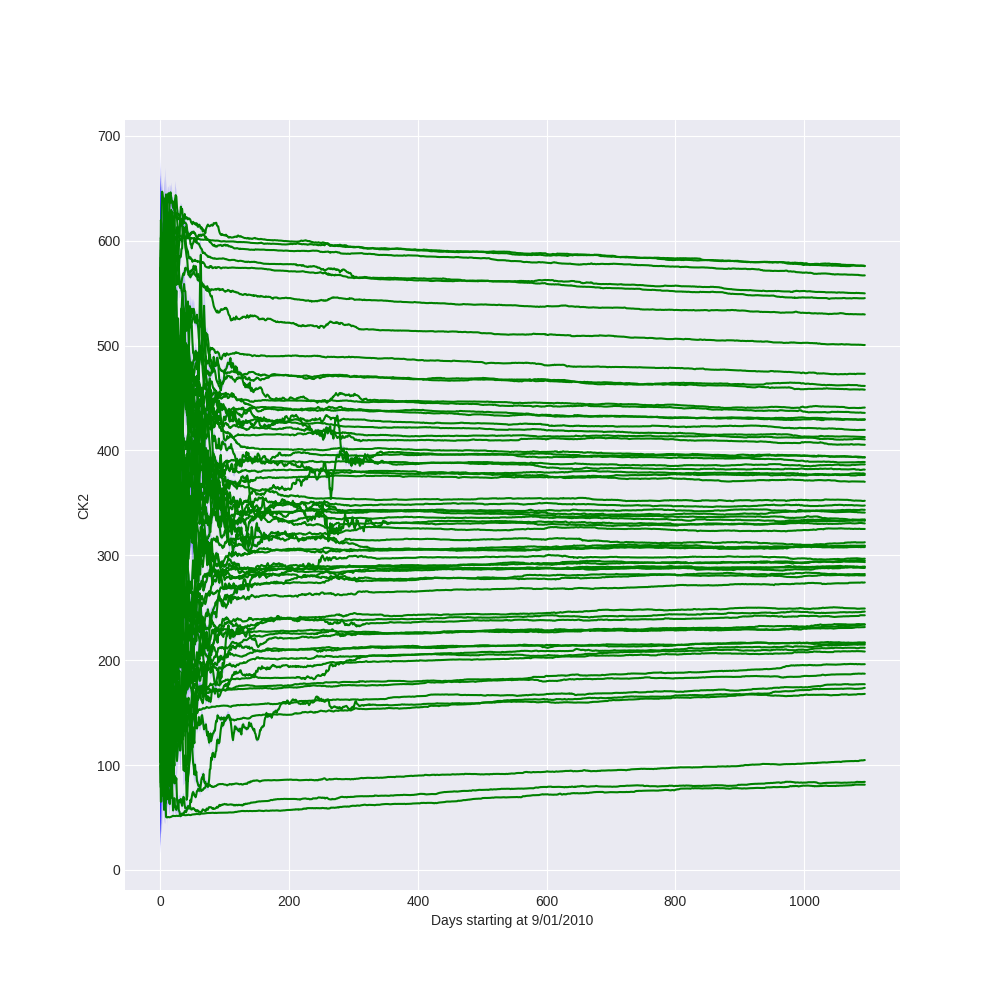
\includegraphics[width = .48\linewidth]{group17streamflow_ck2}} &
\subcaptionbox{\texttt{soil\_beta}\label{2}}{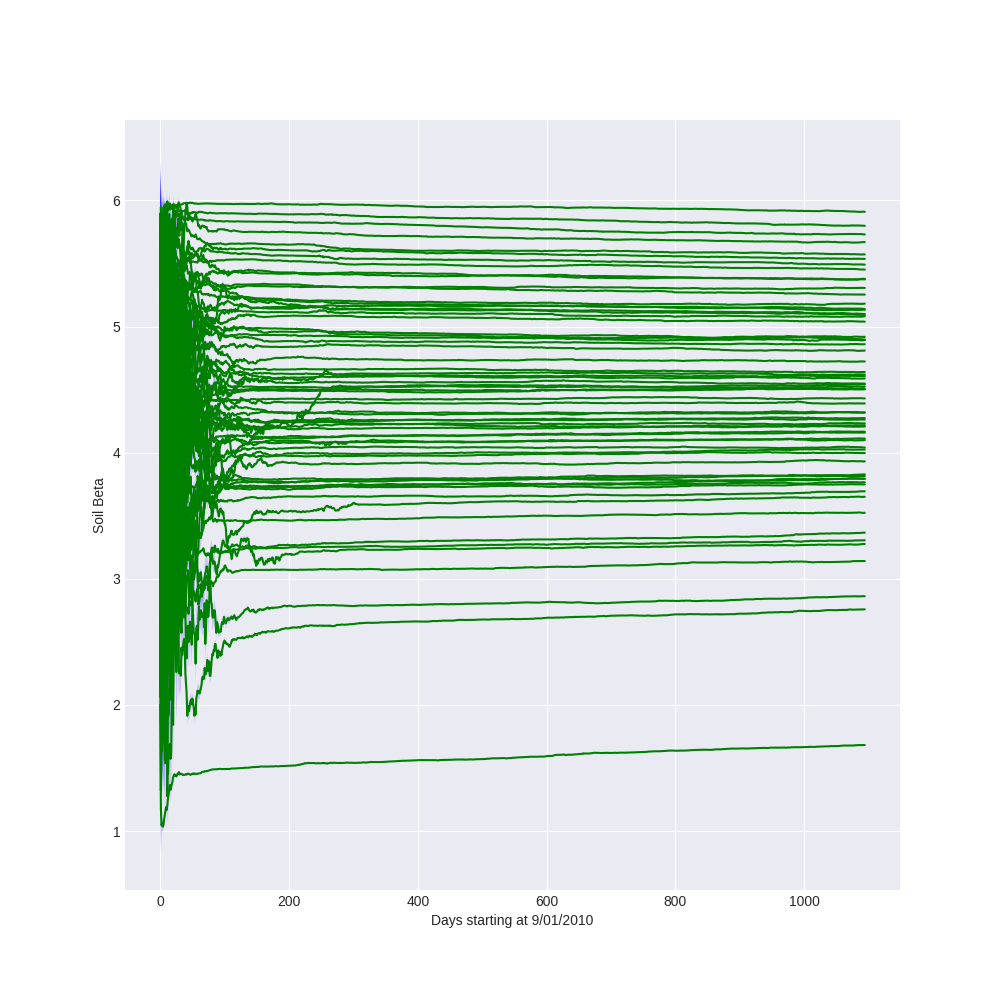
\includegraphics[width = .48\linewidth]{group17streamflow_soil_beta}}

\end{tabular}
\captionof{figure}{All streamflow catchments converged quickly to specific values.}
\label{fig:str_params_cks}
\end{figure}

\begin{figure}
\centering
\begin{minipage}{.48\textwidth}
  \centering
  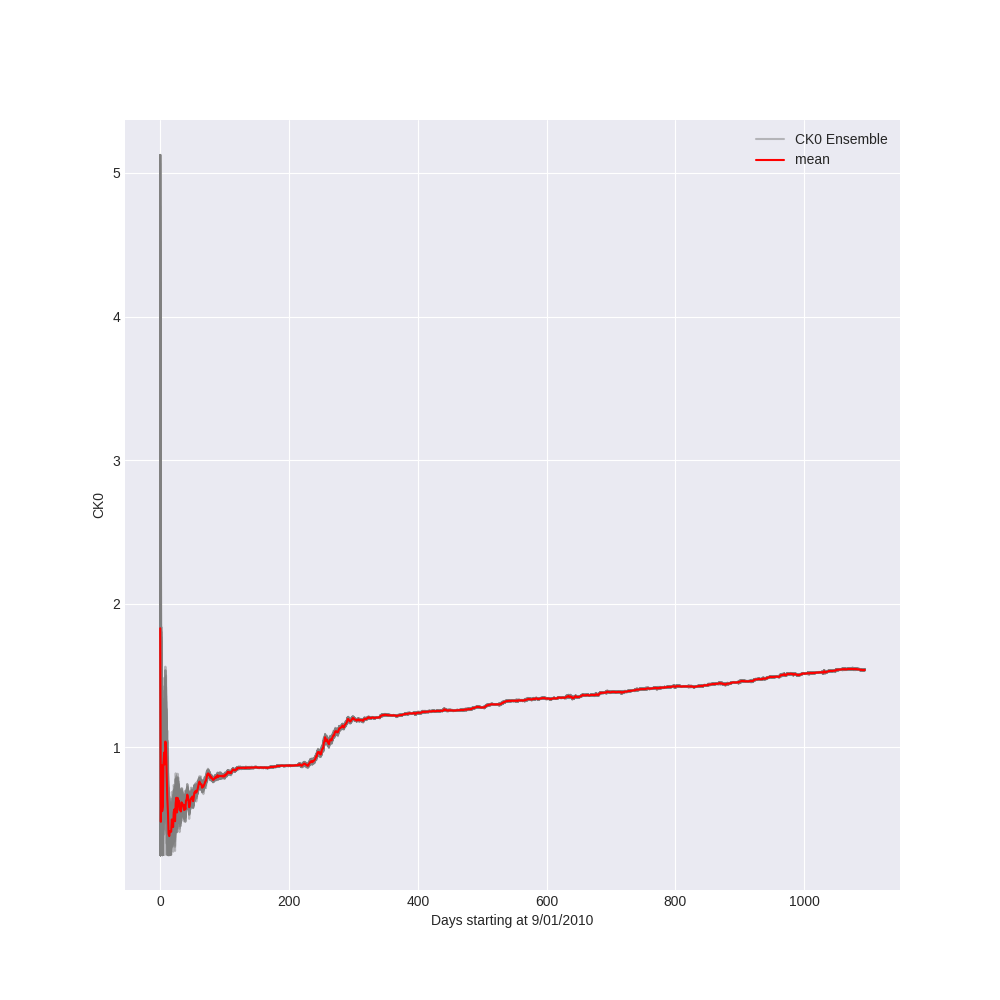
\includegraphics[width=.98\linewidth]{ds_ck0_198}
  \label{fig:ds_ck0_198}
\end{minipage}%
\begin{minipage}{.48\textwidth}
  \centering
  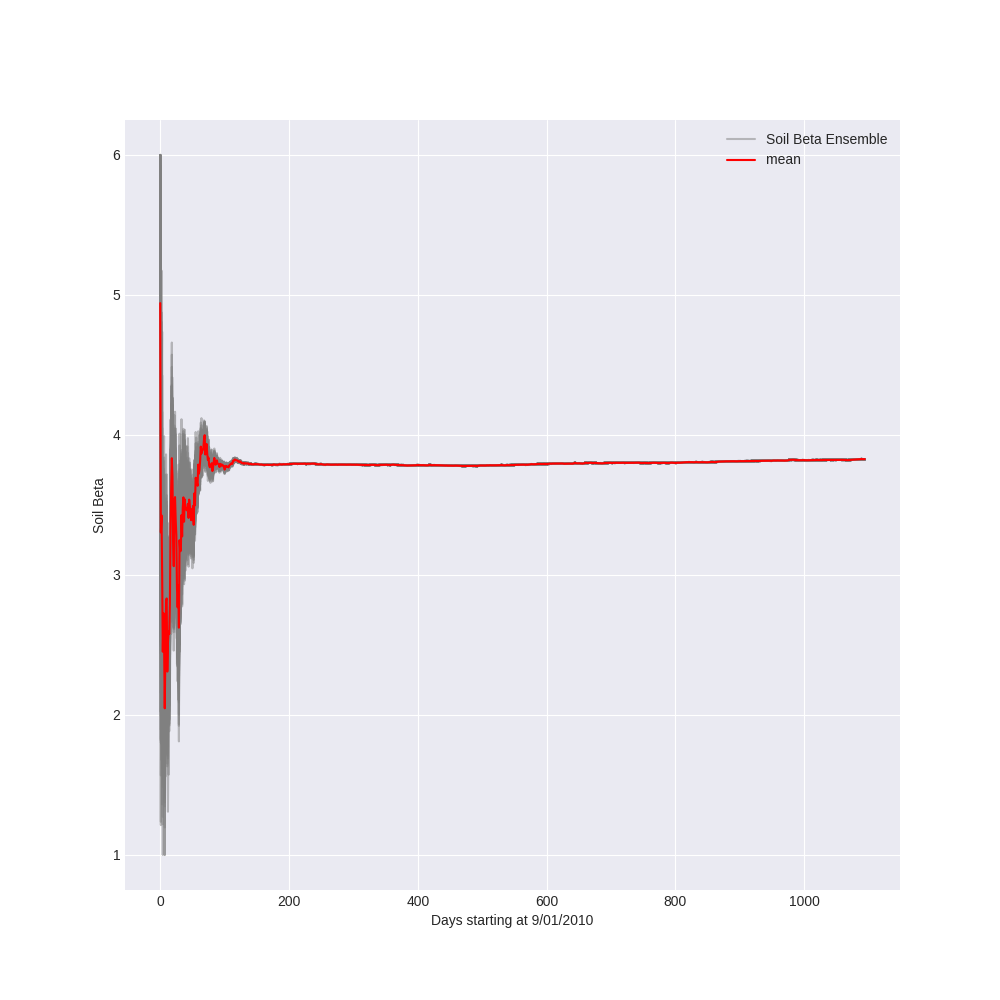
\includegraphics[width=.98\linewidth]{ds_soil_beta_198}
  \label{fig:ds_soil_beta_198}
\end{minipage}
\captionof{figure}{Traces for catchment 198 - \texttt{ck0} and \texttt{soil\_beta}}
\label{fig:str_params_198}
\end{figure}


\subsection{Snow-water equivalent states and parameters}

Snow-water equivalent calibration on the complete dataset behaved similarly to streamflow calibration.

Figure \ref{fig:swe_params} shows the traces for the \texttt{ddf} and \texttt{pp} parameters. These parameters remained locked at their chosen values after the 100th time step. States converged to the observations quickly in gauged nodes (Figure \ref{fig:swe_state} and innovation was generally unbiased (Figure \ref{fig:swe_state_170}.)

\begin{figure}
\centering
\begin{minipage}{.33\textwidth}
  \centering
  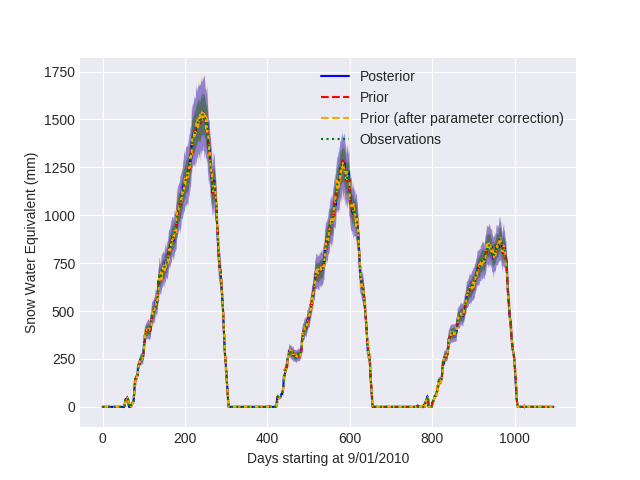
\includegraphics[width=.98\linewidth]{ds_swe_state_42}
  \label{fig:ds_swe_state_42}
\end{minipage}%
\begin{minipage}{.33\textwidth}
  \centering
  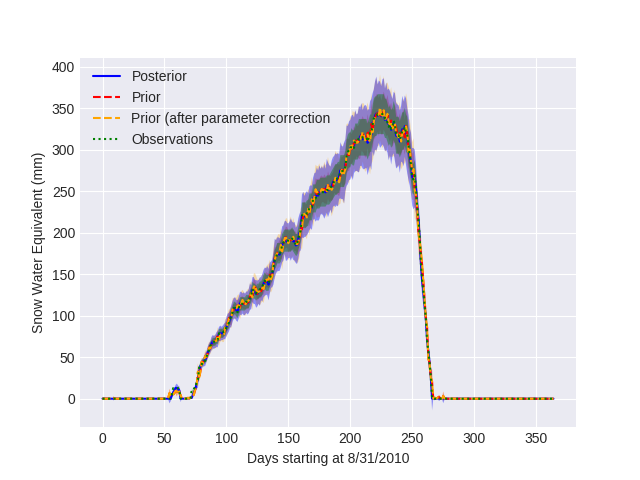
\includegraphics[width=.98\linewidth]{ds_swe_state_241}
  \label{fig:ds_swe_state_241}
\end{minipage}
\begin{minipage}{.33\textwidth}
  \centering
  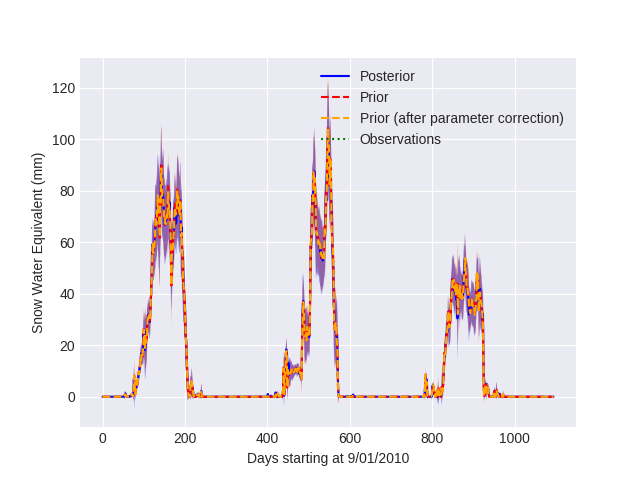
\includegraphics[width=.98\linewidth]{ds_swe_state_137}
  \label{fig:ds_swe_state_137}
\end{minipage}
\captionof{figure}{Snow-water equivalent states for 3 catchments: 42 (gauged), 241 (gauged), and 137 (ungauged)}
\label{fig:swe_state}
\end{figure}

\begin{figure}
\centering
\begin{minipage}{.48\textwidth}
  \centering
  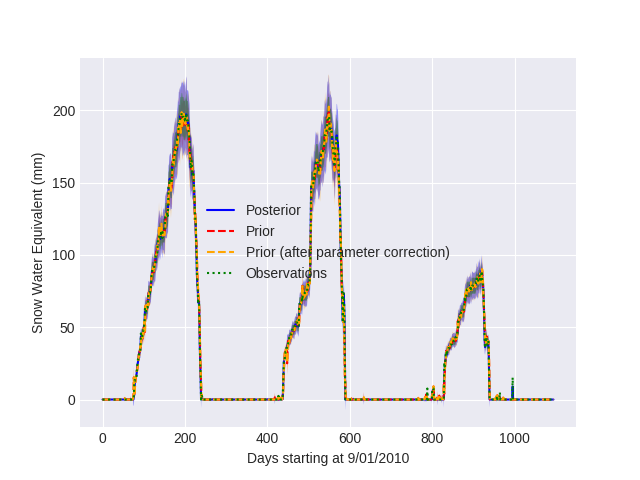
\includegraphics[width=.98\linewidth]{ds_swe_state_170}
  \label{fig:ds_swe_state_170}
\end{minipage}%
\begin{minipage}{.48\textwidth}
  \centering
  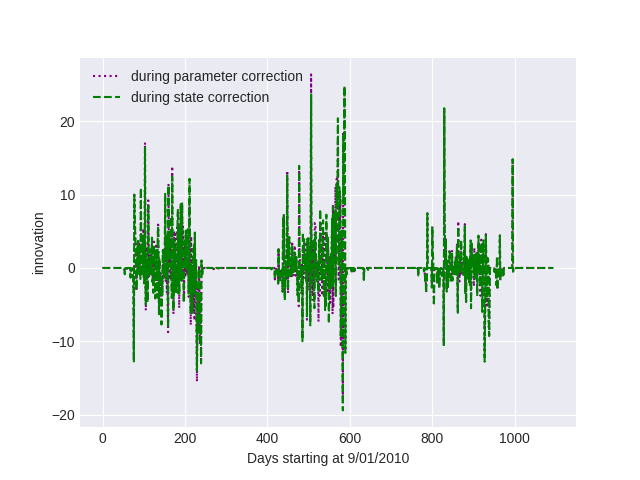
\includegraphics[width=.98\linewidth]{ds_swe_state_170_innovation}
  \label{fig:ds_swe_state_170_innovation}
\end{minipage}
\captionof{figure}{A gauged swe state and its innovation (catchment 170)}
\label{fig:swe_state_170}
\end{figure}

\begin{figure}
\centering
\begin{minipage}{.48\textwidth}
  \centering
  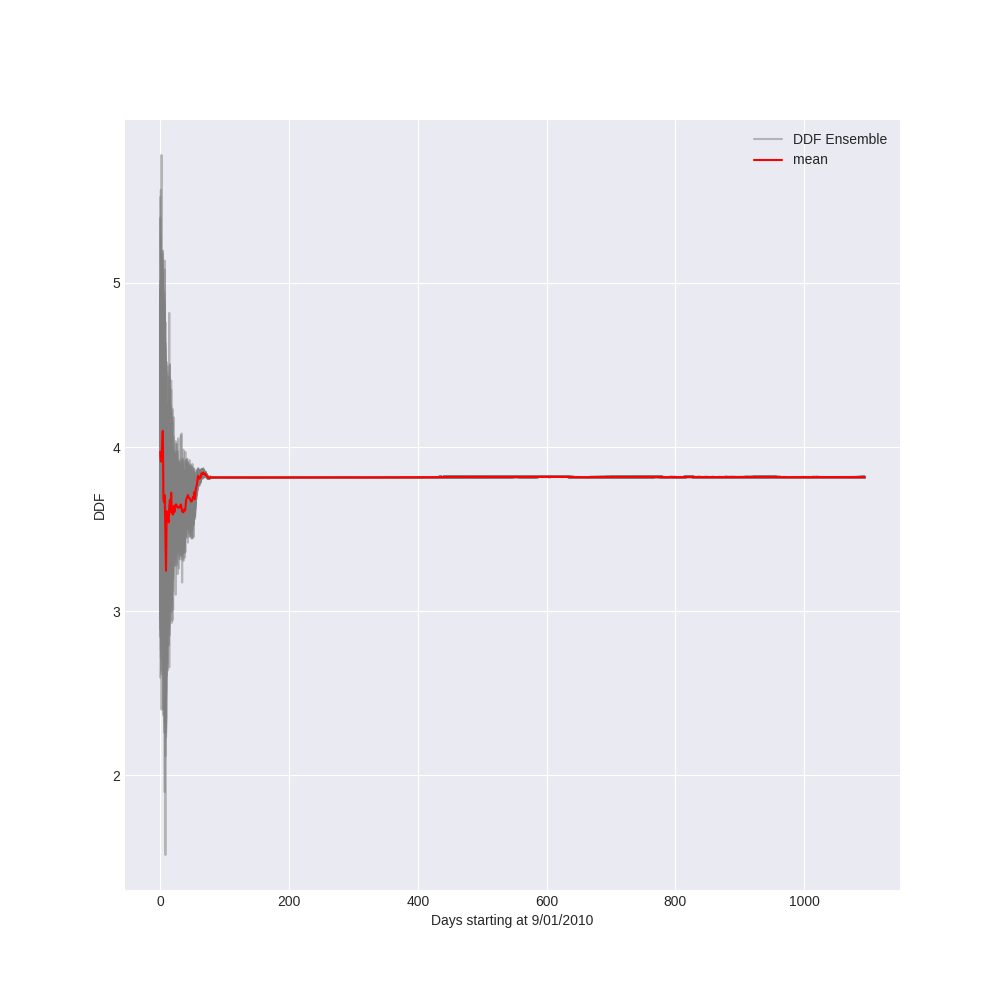
\includegraphics[width=.999\linewidth]{ds_ddf_170}
  \label{fig:ds_ddf_170}
\end{minipage}%
\begin{minipage}{.48\textwidth}
  \centering
  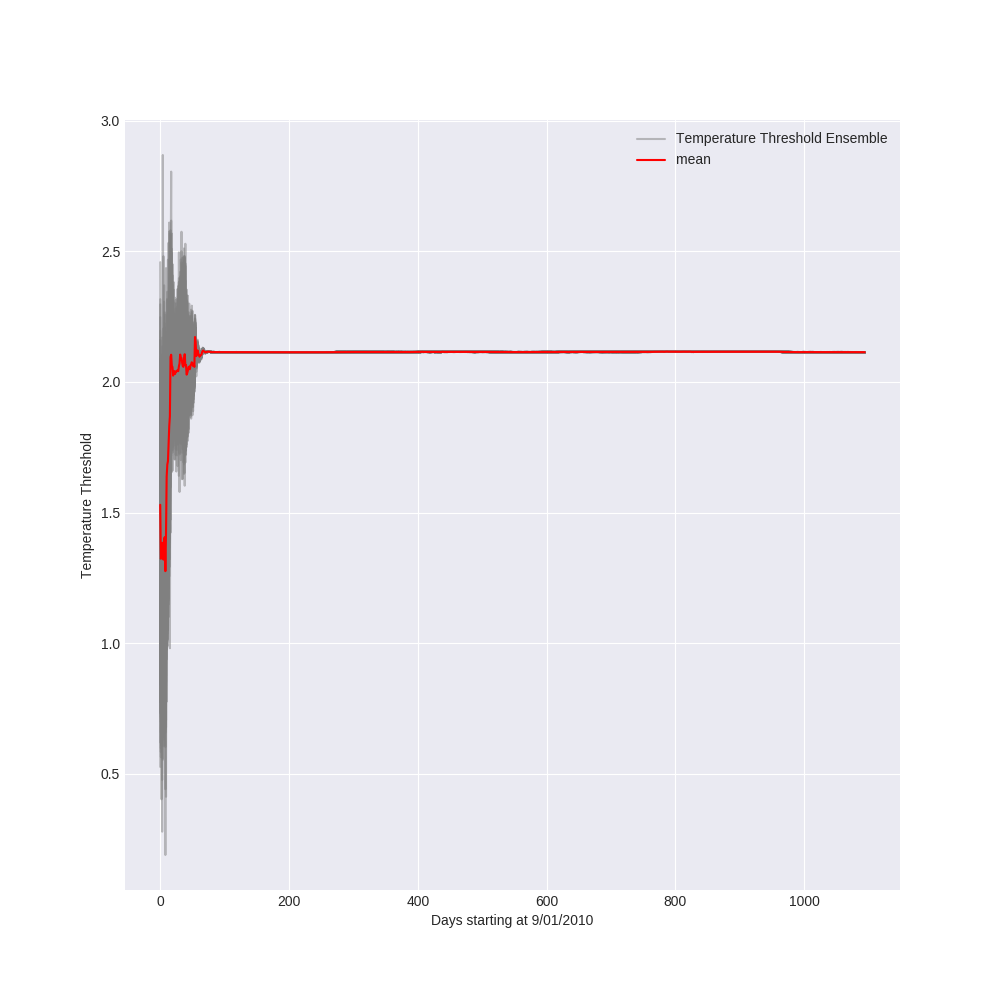
\includegraphics[width=.999\linewidth]{ds_pp_170}
  \label{fig:ds_pp_170}
\end{minipage}
\captionof{figure}{ddf and temperature threshold - catchment 170}
\label{fig:sweparams170}
\end{figure}

\begin{figure}
\begin{tabular}{cc}

\subcaptionbox{\texttt{ddf}\label{2}}{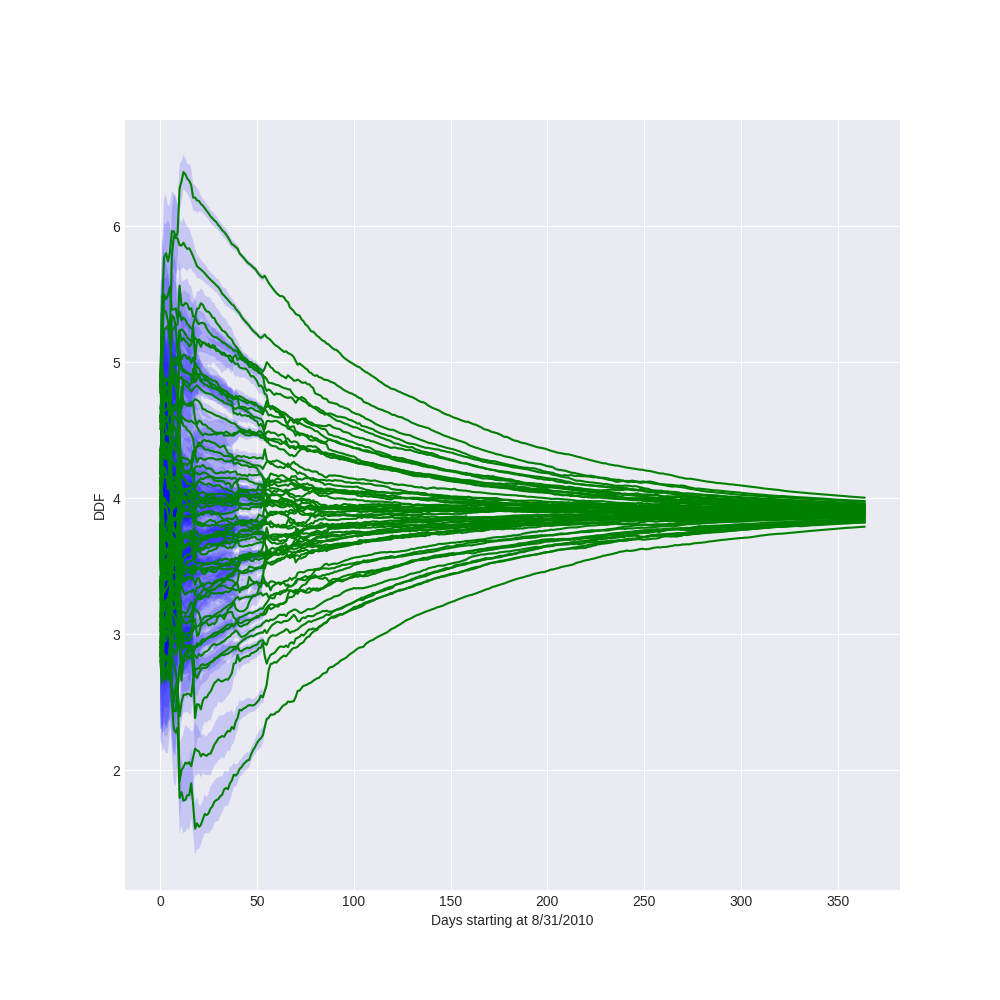
\includegraphics[width = .48\linewidth]{group17swe_ddf}} &
\subcaptionbox{\texttt{pp}\label{2}}{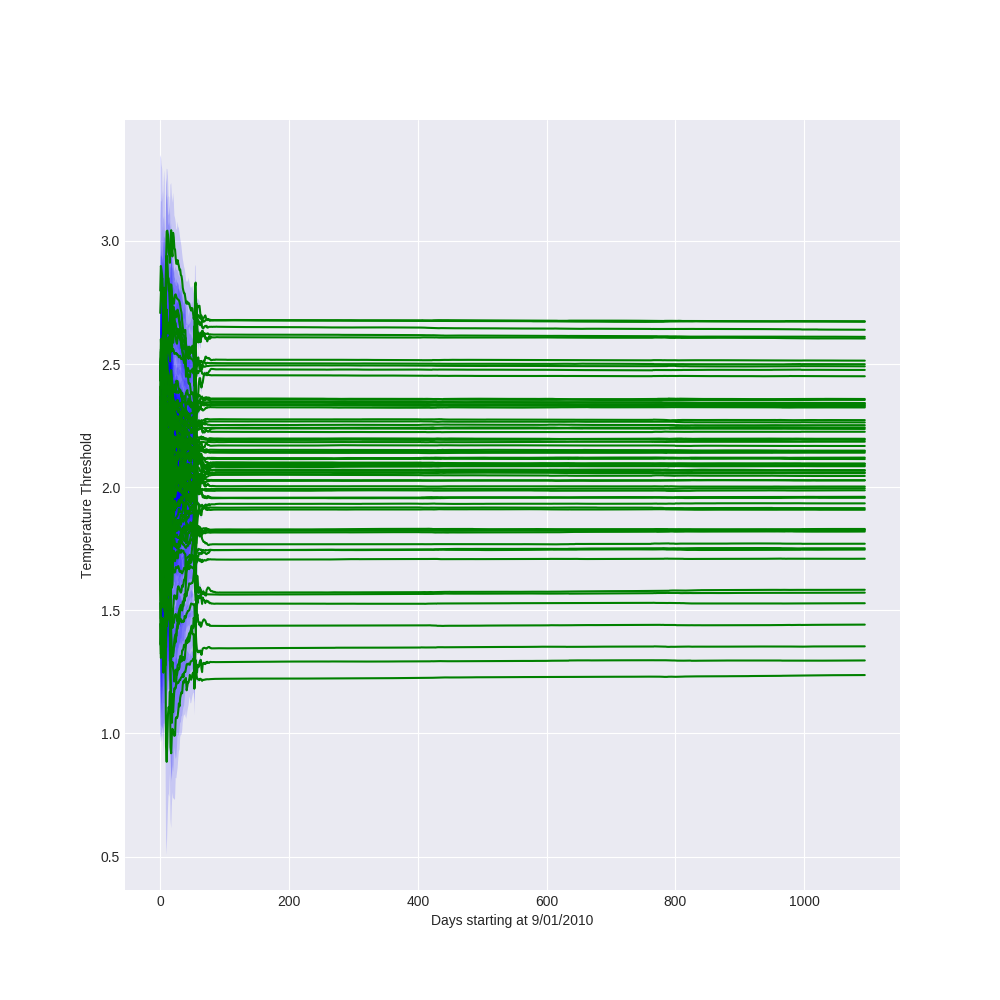
\includegraphics[width = .48\linewidth]{group17swe_pp}}

\end{tabular}
\captionof{figure}{All traces of snow water equivalent related parameters}
\label{fig:swe_params}
\end{figure}

\pagebreak

\section{Effects of the Hierarchical Blending Component}

To observe the effects of the hierarchical component on the filtering process the small dataset was run over 365 timesteps with different values for \texttt{a}. The difference in parameter traces for different values of \texttt{a} may be seen in Figure \ref{fig:hie_params_small}. The value of \texttt{a} controls the maximum amount of weight that may be given to the group mean when ensemble variance as $\lim{var( \theta) \to \infty}$. A very low to nonexistent \texttt{a} value would allow no transfer of data between catchments, while a high \texttt{a} value allows for a complete transfer of information at the expense of temporal memory. For the hydrologic model it was decided that the filter seeks parameters best when \texttt{a} = .9.


\begin{figure}
\begin{tabular}{cc}

\subcaptionbox{\texttt{a} = .1\label{2}}{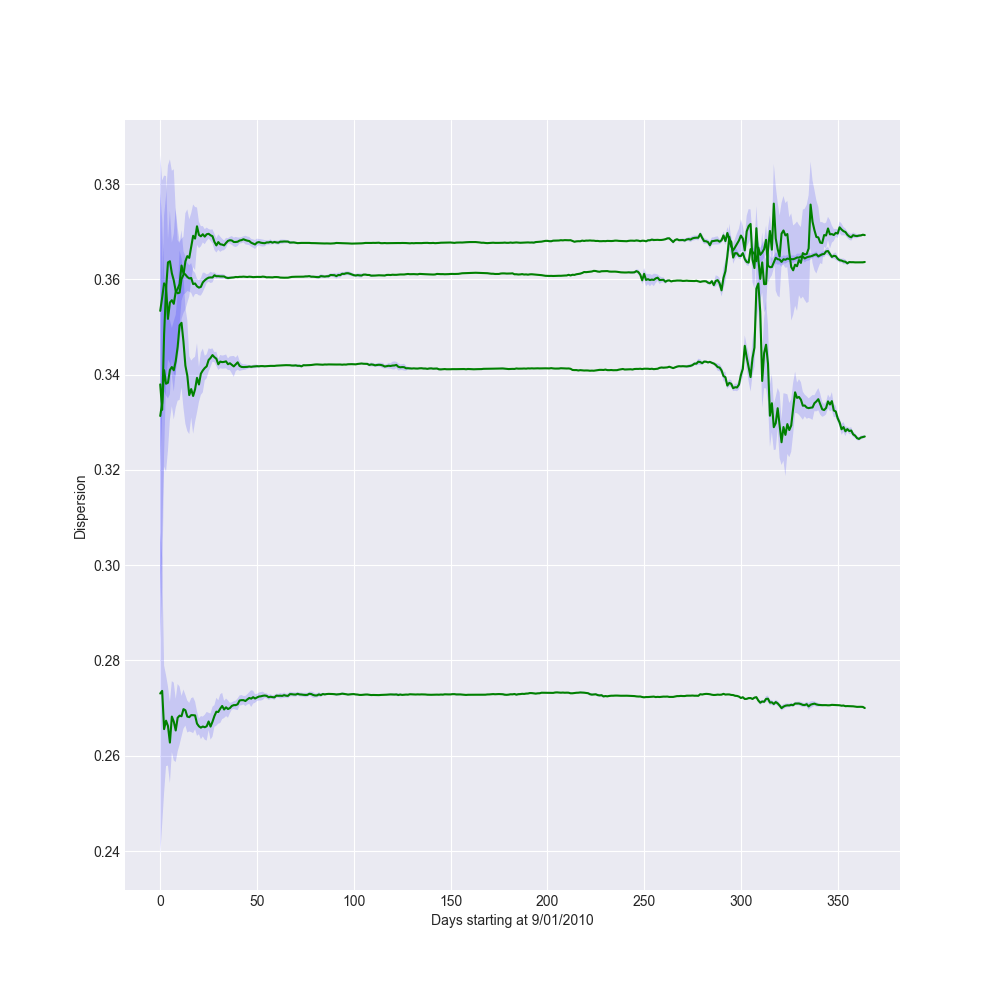
\includegraphics[width = .48\linewidth]{a1}} &
\subcaptionbox{\texttt{a} = .4\label{2}}{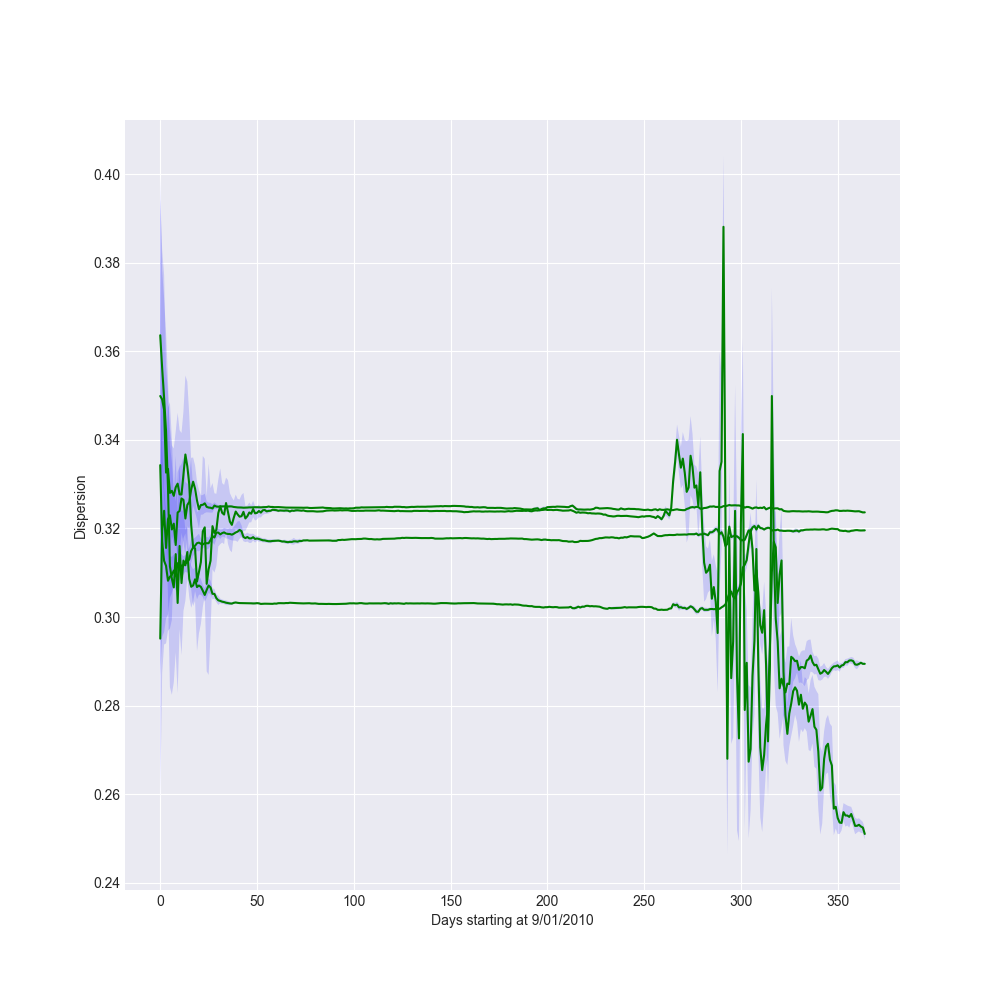
\includegraphics[width = .48\linewidth]{a4}}\\
\subcaptionbox{\texttt{a} = .65\label{2}}{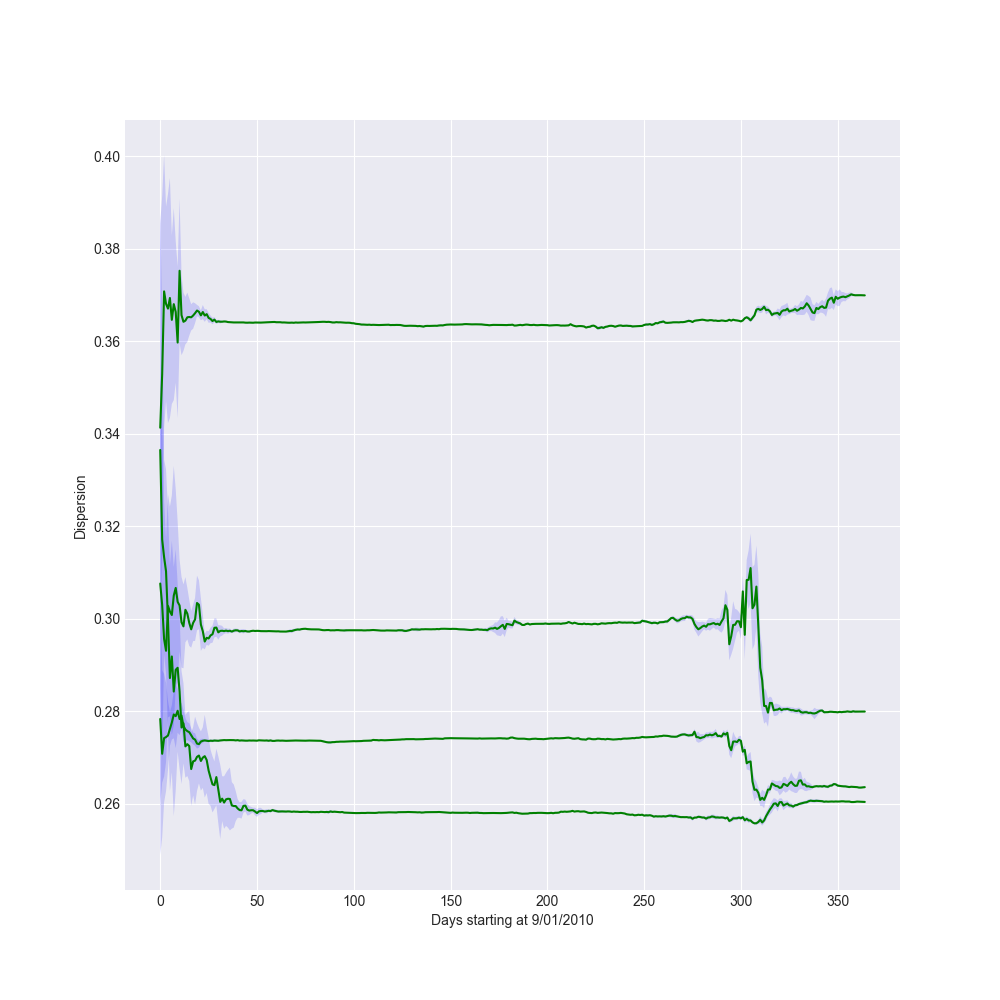
\includegraphics[width = .48\linewidth]{a65}} &
\subcaptionbox{\texttt{a} = .99\label{2}}{\includegraphics[width = .48\linewidth]{a99}}

\end{tabular}
\captionof{figure}{Effect of different values for the blending component \texttt{a}}
\label{fig:hie_params_small}
\end{figure}
